% template presente
\documentclass[a4paper,12pt]{article}

% =======================================================
% 1. CONFIGURAZIONE VARIABILI
% =======================================================
\newcommand{\TitoloDocumento}{Piano di Progetto}
\newcommand{\DataVersione}{AAAA/MM/GG}
\newcommand{\VersioneAttuale}{1.0.0}

% =======================================================
% 2. PACCHETTI
% =======================================================
% Carica xcolor con opzione table (include già colortbl)
\usepackage[table]{xcolor}
\usepackage[utf8]{inputenc}
\usepackage[italian]{babel}
\usepackage{geometry}
\usepackage{graphicx}
\usepackage{float}
\usepackage{setspace}
\usepackage{tabularx} % Per tabelle larghe quanto la pagina
\usepackage{longtable} % Per tabelle su più pagine
\usepackage{fancyhdr} % Per header e footer
\setlength{\headheight}{15pt}
\addtolength{\topmargin}{-2.5pt}
\usepackage{titlesec} % Per formattare i titoli
\setlength{\marginparwidth}{2cm}
\usepackage[colorinlistoftodos]{todonotes}
\usepackage{xurl}     % Per gestire gli url lunghi ed evitare Overfull \hbox
\usepackage{eurosym}
\usepackage{tikz}     % Necessario per i grafici a torta
\usepackage{tcolorbox}

% Percorsi immagini (aggiusta se necessario)
\graphicspath{{resources/}{../resources/}{../../resources/}{../../../resources/}{../../../../resources/}}

% Hyperref va sempre caricato per ultimo
\usepackage{hyperref}
\hypersetup{
    colorlinks=true,
    linkcolor=blue, % Colore link interni
    filecolor=blue,
    urlcolor=blue,  % Colore link web
    pdftitle={\TitoloDocumento},
}

% --- DEFINIZIONE COLORI ---
\definecolor{tableHeader}{RGB}{200, 200, 200}
\definecolor{tableLineOdd}{RGB}{245, 245, 245}
\definecolor{tableLineEven}{RGB}{255, 255, 255}

% Colori per il grafico a torta (ispirati ai ruoli)
\definecolor{pieResp}{RGB}{255, 100, 100} % Rosso chiaro
\definecolor{pieAmm}{RGB}{255, 180, 100}  % Arancione
\definecolor{pieAnal}{RGB}{255, 255, 100}  % Giallo
\definecolor{pieProg}{RGB}{100, 200, 100}  % Verde
\definecolor{pieDes}{RGB}{100, 200, 255}   % Blu chiaro
\definecolor{pieVer}{RGB}{200, 100, 255}   % Viola

% --- DEFINIZIONE COLONNE PERSONALIZZATE ---
\newcolumntype{L}{>{\raggedright\arraybackslash\bfseries}p{4.5cm}}
\newcolumntype{Y}{>{\centering\arraybackslash}X}
\newcolumntype{Z}{>{\raggedright\arraybackslash}X}
% Colonna C definita come X centrata (Necessaria per tabularx)
\newcolumntype{C}{>{\centering\arraybackslash}X}

% =======================================================
% 3. IMPOSTAZIONI VISIVE
% =======================================================
\geometry{margin=2.5cm}
\raggedbottom               % Evita Overfull/Underfull \vbox verticali sulle pagine
\setlength{\parindent}{0pt} % Niente rientro prima riga
\setstretch{1.2}            % Interlinea 1.2

% Stile Header e Footer
\pagestyle{fancy}
\fancyhf{}
\fancyhead[L]{\textcolor{gray}{\TitoloDocumento \ - BitByBit}}
\fancyfoot[C]{\thepage}

% Formattazione Titoli
\titleformat{\section}{\Large\bfseries}{\thesection.}{0.5em}{}
\titleformat{\subsection}{\large\bfseries}{\thesubsection.}{0.5em}{}
\titleformat{\subsubsection}{\bfseries}{\thesubsubsection.}{0.5em}{}

% =======================================================
% 4. INIZIO DOCUMENTO
% =======================================================
\newcommand{\term}[1]{\textbf{#1}$^\mathbf{G}$}

\newcommand{\ignoreglossary}{}

\begin{document}

% --- FRONT PAGE (Loghi e Titoli) ---
\vspace*{\fill}

\begin{center}
    \begin{minipage}{0.25\textwidth}
        \centering
        % Assicurati che il file esista
        
\includegraphics[width=\linewidth]{logoUni.png}
    \end{minipage}
    \hfill
    \begin{minipage}{0.7\textwidth}
        \raggedright
        {\color{red}\LARGE \textbf{Università degli Studi di Padova}}\\[0.3cm]
        {\large
        Laurea: Informatica\\
        Corso: Ingegneria del Software\\
        Anno Accademico: 2025/26
        }
    \end{minipage}
\end{center}

\vspace{1cm}

\begin{center}
    \begin{minipage}{0.25\textwidth}
        \centering
        % Assicurati che il file esista
        
\includegraphics[width=\linewidth]{logo.png}
    \end{minipage}
    \hfill
    \begin{minipage}{0.7\textwidth}
        \raggedright
        {\LARGE \textbf{Gruppo 17}}\\[0.3cm]
        {\large
        Nome: BitByBit\\
        Email: swe.bitbybit@gmail.com
        }
    \end{minipage}
\end{center}

\vspace{1.5cm}

\begin{center}
    {\LARGE \textbf{\TitoloDocumento}}
\end{center}

% ======= INFO GENERALI =======
\renewcommand{\arraystretch}{1.3}

\begin{tcolorbox}
\begin{tabularx}{\textwidth}{@{}l X@{}}
\textbf{Stato:} & Completato\\
\textbf{Versione:} & \VersioneAttuale \\
\textbf{Responsabile:} & Dennis Parolin\\
\textbf{Redattori:} & 
\begin{tabular}[t]{@{}l@{}}
Dennis Parolin\\
Ferdinando Fracasso\\
Marco Sanguin\\
Riccardo Manisi\\
Gabriele Scaggiante\\
\end{tabular} \\
\textbf{Verificatori:} & 
\begin{tabular}[t]{@{}l@{}}
Giovanni Visentin\\
Ferdinando Fracasso\\
Riccardo Manisi\\
Marco Sanguin\\
Gabriele Scaggiante\\
Dennis Parolin\\
\end{tabular} \\
\textbf{Destinatari:} &
\begin{tabular}[t]{@{}l@{}}
Miriade srl\\
Prof. Tullio Vardanega\\
Prof. Riccardo Cardin\\
Gruppo BitByBit\\\\
\end{tabular}
\end{tabularx}
\end{tcolorbox}

\vspace*{\fill}

% =======================================================
% REGISTRO DELLE MODIFICHE
% =======================================================
\clearpage
\section*{Redazione, modifiche e revisioni del documento} \label{sec:registro_modifiche}

\begin{center}
\small
\renewcommand{\arraystretch}{1.4}
\arrayrulecolor{black}

\begin{longtable}{|c|c|>{\raggedright\arraybackslash}p{0.15\linewidth}|>{\raggedright\arraybackslash}p{0.3\linewidth}|c|}
\hline

\rowcolor{gray!60}
\textbf{Versione} & \textbf{Data} & \textbf{Autore} & \textbf{Descrizione} & \textbf{Verificatore} \\
\hline
\endfirsthead

\hline
\rowcolor{gray!60}
\textbf{Versione} & \textbf{Data} & \textbf{Autore} & \textbf{Descrizione} & \textbf{Verificatore} \\
\hline
\endhead
\rowcolor{white}
1.0.0 & 2026-03-03 & Gabriele Scaggiante & Approvazione del documento e stabilizzazione versione del PdP & Dennis Parolin \\
\hline
\rowcolor{gray!20}
0.5.2 & 2026-03-01 & Gabriele Scaggiante & Completata la sezione "\term{Sprint} 7". Fatte correzioni generali e controllo completo dei consuntivi in vista della \term{Milestone} \term{RTB}. & Dennis Parolin \\
\hline
\rowcolor{white}
0.5.1 & 2026-02-25 & Dennis Parolin & Sistemati alcuni errori di visualizzazione. Aggiunto il rischio RO5. Modificati i rischi incontrati dello \term{Sprint} 6 e i rischi attesi dello \term{Sprint} 7. & Ferdinando Fracasso \\
\hline
\rowcolor{gray!20}
0.5.0 & 2026-02-23 & Dennis Parolin & Completata la sezione "\term{Sprint} 6" (\ref{sec:sprint6_RTB}) e fatta la prima metà della sezione "\term{Sprint} 7" (\ref{sec:sprint7_RTB}). Corretti errori di compilazione. & Giovanni Visentin \\
\hline
\rowcolor{white}
0.4.6 & 2026-02-12 & Ferdinando Fracasso & Redazione consuntivo \term{Sprint} nella sezione \ref{sec:sprint4_RTB}, redazione sezione \ref{sec:sprint5_RTB} e inizio sezione \ref{sec:sprint6_RTB} & Marco Sanguin \\
\hline
\rowcolor{gray!20}
0.4.5 & 2026-01-24 & Dennis Parolin & Corretto grafico duplicato & Marco Sanguin \\
\hline
\rowcolor{white}
0.4.4 & 2026-02-03 & Dennis Parolin & Aggiornato il grafico della distribuzione ore per task (figura \ref{fig:distribuzione_ore_rtb}) & Marco Sanguin \\
\hline
\rowcolor{gray!20}
0.4.3 & 2026-01-24 & Dennis Parolin & Aggiunta del grafico con distribuzione ore per task (figura \ref{fig:distribuzione_ore_rtb}) nella sezione di attività previste per la \term{RTB} e sistemate alcune date non presenti nel documento & Gabriele Scaggiante \\
\hline
\rowcolor{white}
0.4.2 & 2026-01-14 & Ferdinando Fracasso & Aggiunte informazioni generali documento nella pagina iniziale & Riccardo Manisi \\
\hline
\rowcolor{gray!20}
0.4.1 & 2026-01-14 & Ferdinando Fracasso & Aggiunte informazioni generali documento nella pagina iniziale & Riccardo Manisi \\
\hline
\rowcolor{white}
0.4.0 & 2026-01-12 & Marco Sanguin & Redazione \ref{sec:sprint2_RTB}, \ref{sec:sprint3_RTB} e inizio \ref{sec:sprint4_RTB} & Dennis Parolin \\
\hline
\rowcolor{gray!20}
0.3.1 & 2026-01-11 & Riccardo Manisi & Aggiunta \ref{tab:RO3} e \ref{tab:RO4}. E aggiunte attività \term{RTB}. & Gabriele Scaggiante \\
\hline
\rowcolor{white}
0.3.0 & 2025-12-05 & Dennis Parolin & Redazione dell'intera sezione \ref{sec:pianificazione_lungo_termine} & Giovanni Visentin \\
\hline
\rowcolor{gray!20}
0.2.0 & 2025-12-04 & Dennis Parolin & Redazione delle sezioni \ref{sec:analisi_rischi} con relative sottosezioni \ref{sec:rischi_tecnologici}, \ref{sec:rischi_organizzativi} e \ref{sec:rischi_interpersonali} & Ferdinando Fracasso \\
\hline
\rowcolor{white}
0.1.0 & 2025-12-03 & Dennis Parolin & Creazione del documento e redazione delle sezioni \ref{sec:scopo_documento}, \ref{sec:definizioni_acronimi_abbreviazioni}, \ref{sec:riferimenti}. & Giovanni Visentin \\
\hline
\end{longtable}
\end{center}

% --- INDICE ---
\clearpage
\tableofcontents
\thispagestyle{empty}
\clearpage

% --- ELENCO TABELLE ---
\listoftables
\clearpage

% =======================================================
% SEZIONE: INTRODUZIONE
% =======================================================

\section{Introduzione}

% =======================SCOPO DOCUMENTO================================
\subsection{Scopo del documento} \label{sec:scopo_documento}
Il \textit{\term{Piano di progetto}} è un documento di natura gestionale che ha lo scopo di definire la pianificazione strategica e operativa delle attività che il gruppo \textit{BitByBit} intraprenderà durante lo sviluppo del progetto didattico.

Il documento è fondamentale per garantire il controllo sull'avanzamento dei lavori e per assicurare il rispetto dei vincoli temporali e qualitativi. In particolare, i suoi obiettivi principali sono:

\begin{itemize}
    \item \textbf{Pianificazione delle attività:} Definire le scadenze interne ed esterne, allocando le risorse temporali necessarie per il completamento di ogni fase.
    \item \textbf{Gestione economica:} Stimare i costi previsti (preventivo) e monitorare i costi effettivi (consuntivo) per ogni periodo di rendicontazione, garantendo la trasparenza verso il \term{Committente}.
    \item \textbf{Analisi e mitigazione dei rischi:} Identificare le potenziali criticità che potrebbero ostacolare lo sviluppo del progetto.
\end{itemize}

Data la natura mutevole dei requisiti e la metodologia agile adottata, il presente documento seguirà un approccio \textbf{incrementale}. Verrà sottoposto a continue revisioni e aggiornamenti al termine di ogni fase significativa del \term{Ciclo di vita} del software, per riflettere lo stato attuale del progetto e affinare le stime future in un'ottica di miglioramento continuo (\textit{continuous improvement}).

% =======================DEFINIZIONI, ACRONIMI E ABBREVIAZIONI================================

\subsection{Definizioni, acronimi e abbreviazioni} \label{sec:definizioni_acronimi_abbreviazioni}

Al fine di evitare ambiguità relative al linguaggio e ai termini utilizzati all'interno dei documenti formali, viene allegato il \href{https://swe-bitbybit.github.io/SWE-docs/docs/RTB/documenti_interni/Glossario.pdf}{\textit{Glossario}}.
I termini tecnici, gli acronimi e le parole con significato specifico all'interno del progetto sono contrassegnati da una lettera 'G' in apice (es. Agile\textsuperscript{G}) e sono descritti in dettaglio nel documento apposito.

% =======================RIFERIMENTI================================

\subsection{Riferimenti} \label{sec:riferimenti}

\subsubsection{Riferimenti normativi}\label{sec:riferimenti_normativi}
\begin{itemize}
\item \textbf{\term{Capitolato} d'appalto C4: \emph{L'app che Protegge e Trasforma}}\\
Parti consultate: documento completo\\
Versione: 1.0.0\\
Ultimo accesso: \textit{2026-01-12}\\
\url{https://www.math.unipd.it/~tullio/IS-1/2025/Progetto/C4.pdf}

\item \textbf{Norme di Progetto}\\
Parti consultate: documento completo\\
Versione: 1.0.0\\
Ultimo accesso: \textit{2026-01-14}\\
\url{} %---Metterei il link nel sito web, ma al momento non è utilizzabile?---
\end{itemize}


\subsubsection{Riferimenti informativi} \label{sec:riferimenti_informativi}
\begin{itemize}
    \item \textbf{Slide sui \emph{processi di \term{Ciclo di vita} del software} del Prof. Vardanega}\\
        Parti consultate: documento completo\\
        Versione: \textit{A.A.2025/2026}\\
        Ultimo accesso: \textit{2026-01-12}\\
        \url{https://www.math.unipd.it/~tullio/IS-1/2025/Dispense/T02.pdf}
    \item \textbf{Slide sulla \emph{gestione di progetto} del Prof. Vardanega}\\
        Parti consultate: documento completo\\
        Versione: \textit{A.A.2025/2026}\\
        Ultimo accesso: \textit{2026-01-12}\\
        \url{https://www.math.unipd.it/~tullio/IS-1/2025/Dispense/T04.pdf}
    \item \textbf{Standard IEEE 830 1998}\\
        Parti consultate: documento completo\\
        Versione: \textit{edizione 1998}\\
        Ultimo accesso: \textit{2026-01-15}\\
        \url{https://ieeexplore.ieee.org/document/720574}
    \item \textbf{Standard ISO/IEC 12207:1995}\\
        Parti consultate: documento completo\\
        Versione: \textit{edizione 1997} \\
        Ultimo accesso: \textit{2026-01-15}\\
        \url{https://www.math.unipd.it/~tullio/IS-1/2009/Approfondimenti/ISO_12207-1995.pdf}
    \item \textbf{Glossario}\\
        Parti consultate: documento completo\\
        Versione: \textit{1.0.0}\\
        Ultimo accesso: \textit{2026-03-03}\\
        \url{https://swe-bitbybit.github.io/SWE-docs/docs/RTB/documenti_interni/Glossario.pdf}
\end{itemize}

% =======================================================
% SEZIONE: ANALISI DEI RISCHI
% =======================================================
\section{Analisi e gestione dei rischi} \label{sec:analisi_rischi}
La gestione del rischio rappresenta una componente nevralgica nella pianificazione di progetto. Questa sezione si prefigge l'obiettivo di individuare preventivamente le potenziali criticità che potrebbero compromettere il rispetto dei vincoli temporali, la qualità del prodotto finale o l'efficienza del team. Una corretta analisi in tal senso è indispensabile per valutare la sostenibilità del carico di lavoro pianificato in relazione alle risorse disponibili.

Il \term{Processo} adottato dal gruppo \textit{BitByBit} segue un approccio sistematico e iterativo, strutturato in quattro fasi distinte che si ripetono ciclicamente durante l'intero \term{Ciclo di vita} del software:

\begin{enumerate}
    \item \textbf{Identificazione:} Ricerca attiva delle potenziali fonti di rischio, analizzando sia aspetti strettamente tecnici che fattori legati all'organizzazione e alla sfera personale dei membri.
    \item \textbf{Analisi:} Valutazione qualitativa e quantitativa dei rischi individuati. Per ciascuna voce viene stimata la probabilità di occorrenza e il potenziale impatto (gravità) sugli obiettivi dello \term{Sprint}\textsuperscript{G} corrente e del progetto globale.
    \item \textbf{Pianificazione:} Definizione proattiva di strategie atte a prevenire l'insorgere del rischio o, qualora la prevenzione totale non fosse possibile, predisposizione di piani di contingenza per mitigarne gli effetti negativi.
    \item \textbf{Controllo:} Monitoraggio costante dello stato del progetto per rilevare tempestivamente l'effettivo verificarsi dei rischi e attivare le contromisure pianificate.
\end{enumerate}

È doveroso sottolineare che, in un contesto didattico caratterizzato da risorse limitate ed esperienza in formazione, le strategie di mitigazione iniziali potrebbero necessitare di affinamenti. Il monitoraggio costante permetterà quindi non solo di arginare i problemi emersi, ma anche di evolvere i processi interni in un'ottica di miglioramento continuo (\textit{continuous improvement}), correggendo eventuali errori di valutazione commessi nelle fasi iniziali.

Per facilitare la gestione e la consultazione, i rischi sono stati catalogati in tre classi principali, ognuna identificata da un codice univoco:
\begin{itemize}
    \item \textbf{RT (Rischi Tecnologici):} Problematiche derivanti dall'adozione di nuovi \term{Framework}, malfunzionamenti hardware o configurazioni software.
    \item \textbf{RO (Rischi Organizzativi):} Criticità legate alla pianificazione, alla stima dei costi, alla distribuzione dei task e alla comprensione dei requisiti.
    \item \textbf{RI (Rischi Interpersonali):} Fattori legati alla disponibilità individuale, agli impegni accademici o lavorativi e alle dinamiche interne al team.
\end{itemize}

% ======================= RISCHI TECNOLOGICI =======================
\clearpage
\subsection{Rischi Tecnologici} \label{sec:rischi_tecnologici}

\subsubsection{RT1 - Inesperienza tecnologica}
\begin{table}[H]
    \centering
    \renewcommand{\arraystretch}{1.4}
    \begin{tabularx}{\textwidth}{|L|Z|}
        \hline
        \rowcolor{tableHeader}
        \textbf{Tipologia Dato} & \textbf{Valore} \\
        \hline
        \rowcolor{tableLineOdd}
        Codice & RT1 \\
        \hline
        \rowcolor{tableLineEven}
        Nome & Inesperienza tecnologica \\
        \hline
        \rowcolor{tableLineOdd}
        Descrizione & Il team potrebbe incontrare difficoltà nell'apprendimento rapido dei \term{Framework} e delle tecnologie richieste dal \term{Capitolato}, causando rallentamenti nello sviluppo. \\
        \hline
        \rowcolor{tableLineEven}
        Mitigazione & Studio individuale approfondito supportato da Proof of Concept (\term{PoC}) preliminari. Adozione di tecniche di \textit{pair programming} per diffondere la conoscenza nel gruppo e livellare le competenze. \\
        \hline
        \rowcolor{tableLineOdd}
        Frequenza probabile & Alta \\
        \hline
        \rowcolor{tableLineEven}
        Pericolosità ripercussioni & Elevata \\
        \hline
    \end{tabularx}
    \caption{Informazioni sul rischio RT1}
    \label{tab:RT1}
\end{table}

\subsubsection{RT2 - Problemi strumenti software}
\begin{table}[H]
    \centering
    \renewcommand{\arraystretch}{1.4}
    \begin{tabularx}{\textwidth}{|L|Z|}
        \hline
        \rowcolor{tableHeader}
        \textbf{Tipologia Dato} & \textbf{Valore} \\
        \hline
        \rowcolor{tableLineOdd}
        Codice & RT2 \\
        \hline
        \rowcolor{tableLineEven}
        Nome & Problemi configurazione strumenti software \\
        \hline
        \rowcolor{tableLineOdd}
        Descrizione & Possibili malfunzionamenti, conflitti di versione o errata configurazione degli ambienti di sviluppo (\term{IDE}, dipendenze) tra i diversi membri del gruppo. \\
        \hline
        \rowcolor{tableLineEven}
        Mitigazione & Standardizzazione dell'ambiente di sviluppo tramite containerizzazione (Docker). Stesura di guide interne per l'installazione e configurazione degli strumenti. \\
        \hline
        \rowcolor{tableLineOdd}
        Frequenza probabile & Media \\
        \hline
        \rowcolor{tableLineEven}
        Pericolosità ripercussioni & Media \\
        \hline
    \end{tabularx}
    \caption{Informazioni sul rischio RT2}
    \label{tab:RT2}
\end{table}

\subsubsection{RT3 - Guasti hardware}
\begin{table}[H]
    \centering
    \renewcommand{\arraystretch}{1.4}
    \begin{tabularx}{\textwidth}{|L|Z|}
        \hline
        \rowcolor{tableHeader}
        \textbf{Tipologia Dato} & \textbf{Valore} \\
        \hline
        \rowcolor{tableLineOdd}
        Codice & RT3 \\
        \hline
        \rowcolor{tableLineEven}
        Nome & Malfunzionamento hardware personale \\
        \hline
        \rowcolor{tableLineOdd}
        Descrizione & Rottura o indisponibilità temporanea del personal computer di un membro del gruppo, con conseguente impossibilità di contribuire allo sviluppo. \\
        \hline
        \rowcolor{tableLineEven}
        Mitigazione & Utilizzo rigoroso del \term{Repository} remoto (GitHub) per il versionamento. Questo garantisce che il lavoro non vada perso e permetta al membro di riprendere il lavoro da una postazione di riserva o universitaria. \\
        \hline
        \rowcolor{tableLineOdd}
        Frequenza probabile & Bassa \\
        \hline
        \rowcolor{tableLineEven}
        Pericolosità ripercussioni & Media \\
        \hline
    \end{tabularx}
    \caption{Informazioni sul rischio RT3}
    \label{tab:RT3}
\end{table}

\subsubsection{RT4 - Introduzione di errori software}
\begin{table}[H]
    \centering
    \renewcommand{\arraystretch}{1.4}
    \begin{tabularx}{\textwidth}{|L|Z|}
        \hline
        \rowcolor{tableHeader}
        \textbf{Tipologia Dato} & \textbf{Valore} \\
        \hline
        \rowcolor{tableLineOdd}
        Codice & RT4 \\
        \hline
        \rowcolor{tableLineEven}
        Nome & Introduzione di bug critici nel codice \\
        \hline
        \rowcolor{tableLineOdd}
        Descrizione & Possibilità che vengano introdotti errori logici o di implementazione (bug) che compromettano le funzionalità già sviluppate o blocchino il progresso del progetto. \\
        \hline
        \rowcolor{tableLineEven}
        Mitigazione & Applicazione rigorosa di Unit Testing e Integration Testing. Obbligo di Code Review ("approvazione") prima di ogni \term{Merge} nel ramo principale. Adozione di pipeline di Continuous Integration (Ci). \\
        \hline
        \rowcolor{tableLineOdd}
        Frequenza probabile & Media \\
        \hline
        \rowcolor{tableLineEven}
        Pericolosità ripercussioni & Alta \\
        \hline
    \end{tabularx}
    \caption{Informazioni sul rischio RT4}
    \label{tab:RT4}
\end{table}

% ======================= RISCHI ORGANIZZATIVI =======================
\subsection{Rischi Organizzativi}\label{sec:rischi_organizzativi}

\subsubsection{RO1 - Errata stima dei costi e tempi}
\begin{table}[H]
    \centering
    \renewcommand{\arraystretch}{1.4}
    \begin{tabularx}{\textwidth}{|L|Z|}
        \hline
        \rowcolor{tableHeader}
        \textbf{Tipologia Dato} & \textbf{Valore} \\
        \hline
        \rowcolor{tableLineOdd}
        Codice & RO1 \\
        \hline
        \rowcolor{tableLineEven}
        Nome & Errata pianificazione temporale \\
        \hline
        \rowcolor{tableLineOdd}
        Descrizione & Rischio di sottostimare o sovrastimare significativamente il tempo necessario per completare un task, portando a scostamenti dal preventivo e ritardi sulla tabella di marcia. \\
        \hline
        \rowcolor{tableLineEven}
        Mitigazione & Monitoraggio continuo a consuntivo per ricalcolare le metriche di produttività. Rimodulazione flessibile dello \term{Sprint backlog} qualora si evidenziassero ritardi. \\
        \hline
        \rowcolor{tableLineOdd}
        Frequenza probabile & Alta \\
        \hline
        \rowcolor{tableLineEven}
        Pericolosità ripercussioni & Media \\
        \hline
    \end{tabularx}
    \caption{Informazioni sul rischio RO1}
    \label{tab:RO1}
\end{table}

\subsubsection{RO2 - Incomprensione dei requisiti}
\begin{table}[H]
    \centering
    \renewcommand{\arraystretch}{1.4}
    \begin{tabularx}{\textwidth}{|L|Z|}
        \hline
        \rowcolor{tableHeader}
        \textbf{Tipologia Dato} & \textbf{Valore} \\
        \hline
        \rowcolor{tableLineOdd}
        Codice & RO2 \\
        \hline
        \rowcolor{tableLineEven}
        Nome & Divergenza sui requisiti \\
        \hline
        \rowcolor{tableLineOdd}
        Descrizione & Possibile errata interpretazione delle richieste del \term{Proponente}, che potrebbe portare allo sviluppo di funzionalità non conformi alle aspettative o inutili. \\
        \hline
        \rowcolor{tableLineEven}
        Mitigazione & Comunicazione frequente e formale con il \term{Proponente} (verbali esterni). Revisione incrociata interna dei documenti di \term{Analisi dei requisiti} prima della \term{Validazione}. \\
        \hline
        \rowcolor{tableLineOdd}
        Frequenza probabile & Bassa \\
        \hline
        \rowcolor{tableLineEven}
        Pericolosità ripercussioni & Elevata \\
        \hline
    \end{tabularx}
    \caption{Informazioni sul rischio RO2}
    \label{tab:RO2}
\end{table}

\subsubsection{RO3 - Incontri non abbastanza frequenti}
\begin{table}[H]
    \centering
    \renewcommand{\arraystretch}{1.4}
    \begin{tabularx}{\textwidth}{|L|Z|}
        \hline
        \rowcolor{tableHeader}
        \textbf{Tipologia Dato} & \textbf{Valore} \\
        \hline
        \rowcolor{tableLineOdd}
        Codice & RO3 \\
        \hline
        \rowcolor{tableLineEven}
        Nome & Incontri non avvenuti \\
        \hline
        \rowcolor{tableLineOdd}
        Descrizione & Gli incontri interni o esterni non avvengono con abbastanza frequenza come si è definito nelle norme di progetto.\\
        \hline
        \rowcolor{tableLineEven}
        Mitigazione & Fissare gli incontri con anticipo di minimo una settimana. Devono essere presenti tutti i componenti del gruppo affinché l'incontro abbia un effetto per l'avanzamento. \\
        \hline
        \rowcolor{tableLineOdd}
        Frequenza probabile & Media \\
        \hline
        \rowcolor{tableLineEven}
        Pericolosità ripercussioni & Elevata \\
        \hline
    \end{tabularx}
    \caption{Informazioni sul rischio RO3}
    \label{tab:RO3}
\end{table}

\subsubsection{RO4 - Assenza di componenti del gruppo}
\begin{table}[H]
    \centering
    \renewcommand{\arraystretch}{1.4}
    \begin{tabularx}{\textwidth}{|L|Z|}
        \hline
        \rowcolor{tableHeader}
        \textbf{Tipologia Dato} & \textbf{Valore} \\
        \hline
        \rowcolor{tableLineOdd}
        Codice & RO4 \\
        \hline
        \rowcolor{tableLineEven}
        Nome & Assenza di un componente \\
        \hline
        \rowcolor{tableLineOdd}
        Descrizione & Comunicazione assente per un periodo di tempo maggiore di una settimana da parte di un componente del gruppo, con anche mancata presenza agli incontri interni svolti. Mancato completamento delle attività assegnate.\\
        \hline
        \rowcolor{tableLineEven}
        Mitigazione & Nessuna. \\
        \hline
        \rowcolor{tableLineOdd}
        Frequenza probabile & Bassa \\
        \hline
        \rowcolor{tableLineEven}
        Pericolosità ripercussioni & Media \\
        \hline
    \end{tabularx}
    \caption{Informazioni sul rischio RO4}
    \label{tab:RO4}
\end{table}

\subsubsection{RO5 - Dipendenza da risorse e permessi esterni}
\begin{table}[H]
    \centering
    \renewcommand{\arraystretch}{1.4}
    \begin{tabularx}{\textwidth}{|L|Z|}
        \hline
        \rowcolor{tableHeader}
        \textbf{Tipologia Dato} & \textbf{Valore} \\
        \hline
        \rowcolor{tableLineOdd}
        Codice & RO5 \\
        \hline
        \rowcolor{tableLineEven}
        Nome & Mancanza o ritardo nella fornitura di permessi e risorse esterne \\
        \hline
        \rowcolor{tableLineOdd}
        Descrizione & Lo sviluppo del progetto può richiedere l'utilizzo di specifiche risorse, piattaforme (es. \term{Cloud}) o credenziali fornite direttamente dall'azienda \term{Proponente}. Eventuali ritardi nella fornitura di tali strumenti o la mancanza iniziale dei permessi necessari possono causare blocchi temporanei nelle normali attività di sviluppo e test, incidendo sulla tempistica dello \term{Sprint}. \\
        \hline
        \rowcolor{tableLineEven}
        Mitigazione & Individuazione tempestiva e proattiva delle necessità tecniche per comunicarle prontamente all'azienda \term{Proponente}. In caso di attesa prolungata, riorganizzazione flessibile ed elastica dei task dello \term{Sprint} in modo da portare avanti le attività parallele e indipendenti dalle risorse bloccate, riducendo al minimo i tempi morti. \\
        \hline
        \rowcolor{tableLineOdd}
        Frequenza probabile & Media \\
        \hline
        \rowcolor{tableLineEven}
        Pericolosità ripercussioni & Elevata \\
        \hline
    \end{tabularx}
    \caption{Informazioni sul rischio RO5}
    \label{tab:RO5}
\end{table}

% ======================= RISCHI INTERPERSONALI =======================
\subsection{Rischi Interpersonali}\label{sec:rischi_interpersonali}

\subsubsection{RI1 - Impegni accademici}
\begin{table}[H]
    \centering
    \renewcommand{\arraystretch}{1.4}
    \begin{tabularx}{\textwidth}{|L|Z|}
        \hline
        \rowcolor{tableHeader}
        \textbf{Tipologia Dato} & \textbf{Valore} \\
        \hline
        \rowcolor{tableLineOdd}
        Codice & RI1 \\
        \hline
        \rowcolor{tableLineEven}
        Nome & Concomitanza impegni accademici \\
        \hline
        \rowcolor{tableLineOdd}
        Descrizione & La presenza di appelli d'esame, progetti di altri corsi o lezioni obbligatorie può ridurre drasticamente la disponibilità oraria dei membri in periodi critici. \\
        \hline
        \rowcolor{tableLineEven}
        Mitigazione & Pianificazione a lungo termine che evidenzi le date degli appelli nel calendario condiviso. Riduzione del carico di lavoro previsto negli \term{Sprint} coincidenti con le sessioni d'esame. \\
        \hline
        \rowcolor{tableLineOdd}
        Frequenza probabile & Alta \\
        \hline
        \rowcolor{tableLineEven}
        Pericolosità ripercussioni & Elevata \\
        \hline
    \end{tabularx}
    \caption{Informazioni sul rischio RI1}
    \label{tab:RI1}
\end{table}

\subsubsection{RI2 - Problemi personali}
\begin{table}[H]
    \centering
    \renewcommand{\arraystretch}{1.4}
    \begin{tabularx}{\textwidth}{|L|Z|}
        \hline
        \rowcolor{tableHeader}
        \textbf{Tipologia Dato} & \textbf{Valore} \\
        \hline
        \rowcolor{tableLineOdd}
        Codice & RI2 \\
        \hline
        \rowcolor{tableLineEven}
        Nome & Indisponibilità per motivi personali \\
        \hline
        \rowcolor{tableLineOdd}
        Descrizione & Imprevisti di salute, familiari o lavorativi che impediscono a un membro di lavorare per un periodo limitato o esteso. \\
        \hline
        \rowcolor{tableLineEven}
        Mitigazione & Comunicazione tempestiva al Responsabile. Ridistribuzione dinamica dei task urgenti tra gli altri componenti (uso di \textit{slack} temporale). \\
        \hline
        \rowcolor{tableLineOdd}
        Frequenza probabile & Bassa \\
        \hline
        \rowcolor{tableLineEven}
        Pericolosità ripercussioni & Media \\
        \hline
    \end{tabularx}
    \caption{Informazioni sul rischio RI2}
    \label{tab:RI2}
\end{table}

\subsubsection{RI3 - Contrasti interni}
\begin{table}[H]
    \centering
    \renewcommand{\arraystretch}{1.4}
    \begin{tabularx}{\textwidth}{|L|Z|}
        \hline
        \rowcolor{tableHeader}
        \textbf{Tipologia Dato} & \textbf{Valore} \\
        \hline
        \rowcolor{tableLineOdd}
        Codice & RI3 \\
        \hline
        \rowcolor{tableLineEven}
        Nome & Conflitti nel gruppo \\
        \hline
        \rowcolor{tableLineOdd}
        Descrizione & Divergenze di opinioni tecniche o metodologiche, oppure tensioni interpersonali che rallentano il \term{Processo} decisionale e minano la serenità del gruppo. \\
        \hline
        \rowcolor{tableLineEven}
        Mitigazione & Promozione di un clima di dialogo aperto. Intervento del Responsabile di Progetto come mediatore. Adozione di sistemi di votazione democratica per le decisioni bloccanti. \\
        \hline
        \rowcolor{tableLineOdd}
        Frequenza probabile & Bassa \\
        \hline
        \rowcolor{tableLineEven}
        Pericolosità ripercussioni & Elevata \\
        \hline
    \end{tabularx}
    \caption{Informazioni sul rischio RI3}
    \label{tab:RI3}
\end{table}

%============================================== 
%       PIANIFICAZIONE NEL LUNGO TERMINE
%==============================================
\section{Pianificazione nel lungo termine}\label{sec:pianificazione_lungo_termine}

\subsection{Introduzione}
Come dichiarato nel documento di \href{https://swe-bitbybit.github.io/SWE-docs/docs/candidatura/valutazione_costi_rischi/valutazione_costi_rischi.pdf}{valutazione costo e rischi}, il gruppo si impegna a terminare il progetto entro e non oltre il giorno \textbf{2026-04-15} con un budget di spesa fissato a \textbf{11.370\euro}.

Nella fase di candidatura si è teorizzato il seguente prospetto di ripartizione oraria e dei costi:

\begin{table}[H]
    \centering
    \renewcommand{\arraystretch}{1.5}
    \begin{tabularx}{\textwidth}{|c|C|C|C|}
        \hline
        \rowcolor{tableHeader}
        \textbf{Ruolo} & \textbf{Costo Orario} & \textbf{Ore Totali} & \textbf{Costo Totale} \\
        \hline
        \rowcolor{tableLineOdd}
        Responsabile & 30€/h & 78 & 2.340\euro \\
        \hline
        \rowcolor{tableLineEven}
        Amministratore & 20€/h & 84 & 1.680\euro \\
        \hline
        \rowcolor{tableLineOdd}
        Analista & 25€/h & 66 & 1.650\euro \\
        \hline
        \rowcolor{tableLineEven}
        Progettista & 25€/h & 102 & 2.550\euro \\
        \hline
        \rowcolor{tableLineOdd}
        Programmatore & 15€/h & 120 & 1.800\euro \\
        \hline
        \rowcolor{tableLineEven}
        Verificatore & 15€/h & 90 & 1.350\euro \\
        \hline
        \rowcolor{tableHeader}
        \textbf{Totale} & - & \textbf{540} & \textbf{ 11.370\euro } \\
        \hline
    \end{tabularx}
    \caption{Preventivo iniziale teorizzato in fase di candidatura}
    \label{tab:preventivo_candidatura}
\end{table}

Si stima inoltre una candidatura per la \textbf{Requirements and Technology \term{Baseline} (\term{RTB})} entro il \textbf{2026-02-12}.

% ======================= ATTIVITA PREVISTE PER \term{RTB} =======================
\subsection{Attività previste per la Requirements and Technology Baseline (Rtb)}

\begin{table}[H]
    \centering
    \renewcommand{\arraystretch}{1.5}
    \arrayrulecolor{black}
    \begin{tabularx}{\textwidth}{|L|Z|}
        \hline
        \rowcolor{tableHeader}
        \textbf{Attività} & \textbf{Descrizione} \\
        \hline
        \rowcolor{tableLineOdd}
        Redazione norme di Progetto & Definisce le regole, le convenzioni e gli strumenti che regolano il \textit{\term{Way of working}} del team, assicurando uniformità e coerenza nello svolgimento delle attività. \\
        \hline
        \rowcolor{tableLineEven}
        Implementazione Sito & Implementazione del sito per facilitare la fruizione dei documenti prodotti dal gruppo durante i processi di \term{Ciclo di vita}. \\
        \hline
        \rowcolor{tableLineOdd}
        Redazione del \term{Piano di progetto} & Pianifica le risorse, i costi e le scadenze temporali, delineando le attività passate, presenti e future per garantire il rispetto degli obiettivi prefissati. \\
        \hline
        \rowcolor{tableLineEven}
        Redazione del \term{Piano di qualifica} & Stabilisce le metriche e le procedure di controllo necessarie per verificare la qualità dei processi e del prodotto software durante l'intero \term{Ciclo di vita}. \\
        \hline
        \rowcolor{tableLineOdd}
        Implementazione del cruscotto di valutazione & Implementazione del cruscotto per l'accertamento della qualità tramite lo strumento scelto dal gruppo. Riporta le misurazioni e le loro valutazioni per una migliore comprensione. \\
        \hline
        \rowcolor{tableLineEven}
        Redazione casi d'uso per AdR & Scrittura della sezione del documento \term{Analisi dei requisiti} relativa ai casi d'uso. \\
        \hline
        \rowcolor{tableLineEven}
        Redazione requisiti per AdR & Implementazione della sezione del documento \term{Analisi dei requisiti} relativa ai requisiti del prodotto software. \\
        \hline
        \rowcolor{tableLineEven}
        Redazione \term{Analisi dei requisiti} & Formalizza i requisiti funzionali, non funzionali e di vincolo concordati con il \term{Proponente}, dettagliando i casi d'uso del sistema. \\
        \hline
        \rowcolor{tableLineEven}
        Realizzazione del Proof of Concept & Prototipo software volto a verificare la fattibilità tecnica della soluzione e l'efficacia delle tecnologie selezionate per lo sviluppo. Utilizzato anche per familiarizzare con le tecnologie proposte. \\
        \hline
        \rowcolor{tableLineOdd}
        Lettera di presentazione \term{RTB} & Documento formale che accompagna la consegna, ufficializzando la richiesta del gruppo di sostenere la revisione \textit{Requirements and Technology \term{Baseline}}. \\
        \hline
    \end{tabularx}
    \caption{Attività previste per la \term{RTB}}
    \label{tab:attivita_rtb}
\end{table}

Per le fasi di \textbf{Requirements and Technology \term{Baseline} (\term{RTB})} e \textbf{Product \term{Baseline} (\term{PB})} sono state definite delle attività specifiche da completare. Queste sono fondamentali per una corretta gestione degli \term{Sprint} che verranno eseguiti. Di seguito sono elencate le attività previste:

Per garantire una corretta distribuzione del carico di lavoro e rispettare le scadenze previste per la \term{RTB}, è stata effettuata una stima dettagliata delle ore necessarie per ogni ruolo, suddivise per task specifici. Questa analisi permette di evidenziare come le diverse attività impattino sull'impegno complessivo dei membri del team.
Il grafico seguente (Figura \ref{fig:distribuzione_ore_rtb}) illustra visivamente il monte ore totale previsto per ciascun ruolo nella fase di \term{RTB}, evidenziando tramite i diversi colori il contributo delle singole attività al carico di lavoro complessivo.

In particolare, per stimare le ore del Verificatore visibili nel grafico, è stato deciso di calcolarle come il 20\% delle ore previste per quella specifica task. Ad esempio, se l'attività \textbf{Redazione verbali} occupa 17 ore del Responsabile, la relativa \term{Verifica} è stimata in 3.4 ore. È importante notare che questa è solo una stima: eventuali ore risparmiate su alcune task potranno essere sfruttate per la \term{Verifica} di altre attività.

\begin{figure}[H]
    \centering
    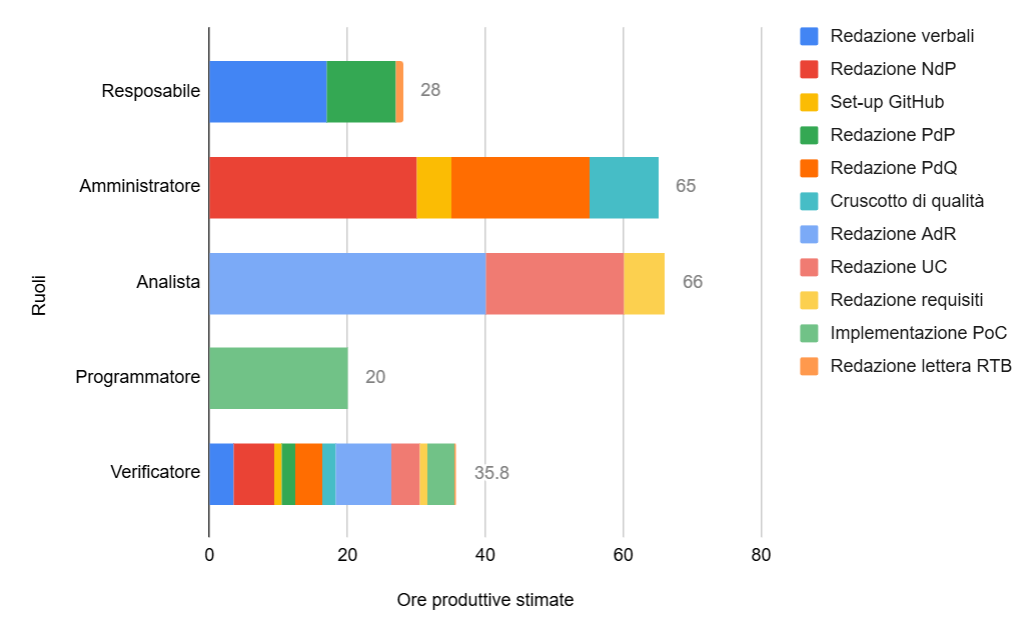
\includegraphics[width=\textwidth]{../../../../resources/distribuzione_ore_rtb.png}
    \caption{Distribuzione ore produttive stimate per ruolo e attività - \term{RTB}}
    \label{fig:distribuzione_ore_rtb}
\end{figure}

% ======================= ATTIVITA PREVISTE PER \term{PB} =======================
\subsection{Attività previste per la Product Baseline (Pb)}
La redazione di questo paragrafo sarà effettuato in seguito al superamento della
\textbf{Requirements and Technology \term{Baseline} (\term{RTB})}.


%============================================== 
%       PIANIFICAZIONE NEL BREVE TERMINE
%==============================================

\section{Pianificazione nel breve termine}\label{sec:pianificazione_breve_termine}

% ======================= INTRODUZIONE =======================
\subsection{Introduzione}
Il gruppo \textit{BitByBit} ha scelto di organizzare lo sviluppo del progetto seguendo un modello iterativo e incrementale, ispirato ai principi della metodologia \textbf{Agile}. Il lavoro sarà suddiviso in unità temporali denominate \textit{\term{Sprint}}, ciascuno con una durata due settimane.

Questa strategia permette di mantenere una pianificazione flessibile e adattiva. All'inizio di ogni iterazione, il gruppo definirà gli obiettivi a breve termine e assegnerà le attività, prevedendo una \textbf{rotazione dei ruoli}. Tale rotazione è fondamentale per garantire che ogni membro del team acquisisca competenze trasversali e abbia visione completa del \term{Processo} produttivo.

Elemento cardine del metodo di lavoro sarà il confronto con il \term{Proponente}, l'azienda \textbf{Miriade}. Sono previsti incontri online su \textbf{Google Meet} o con il canale indiretto concordato (\textbf{Google Chat}) per verificare la conformità di quanto prodotto rispetto alle aspettative.

Per ogni \term{Sprint} descritto in questa sezione, verranno riportate le seguenti informazioni:
\begin{itemize}
    \item \textbf{Obiettivi e attività:} Descrizione delle finalità dello \term{Sprint} e delle task pianificate.
    \item \textbf{Gestione dei rischi:} Analisi dei rischi specifici che potrebbero manifestarsi nel periodo considerato.
    \item \textbf{Rendicontazione:} Prospetto preventivo delle ore e dei costi stimati, seguito dal consuntivo finale con l'analisi degli eventuali scostamenti.
\end{itemize}

% ======================= \term{RTB} =======================
\subsection{Requirements and Technology Baseline (Rtb)}

\subsubsection{Sprint 1}\label{sec:sprint1_RTB}

% --- TABELLA RIEPILOGATIVA \term{Sprint} ---
\begin{table}[H]
    \centering
    \renewcommand{\arraystretch}{1.5}
    \begin{tabularx}{\textwidth}{|>{\columncolor{tableHeader}\bfseries}l|X|>{\columncolor{tableHeader}\bfseries}l|X|}
        \hline
        Inizio & 2025-11-19 & Fine prevista & 2025-12-03 \\
        \hline
        Stato & \textbf{Concluso} & Fine reale & 2025-12-03 \\
        \hline
        \multicolumn{2}{|c|}{\cellcolor{tableHeader}\textbf{Giorni di ritardo}} & \multicolumn{2}{c|}{0} \\
        \hline
    \end{tabularx}
    \caption{Riepilogo temporale \term{Sprint} 1}
\end{table}

\paragraph{Informazioni generali e attività da svolgere}
Lo \term{Sprint} 1 ha rappresentato l'avvio operativo del progetto. L'obiettivo primario era la definizione delle funzionalità da proporre al \term{Committente} e l'avvio della produzione documentale, oltre all'organizzazione interna del gruppo (ruoli e strumenti).

Le attività pianificate e svolte includono:
\begin{itemize}
    \item \textit{Analisi:} Studio del \term{Capitolato} e selezione delle funzionalità chiave.
    \item \textit{Incontri:} Preparazione delle domande per il primo meeting con Miriade.
    \item \textit{Documentazione:} Avvio della stesura dei documenti \textit{\term{Analisi dei requisiti}} (AdR), \textit{Norme di Progetto} (NdP) e \textit{\term{Piano di progetto}} (PdP).
    \item \textit{Gestione:} Discussione e assegnazione dei ruoli.
\end{itemize}

\paragraph{Rischi attesi}
Per questo \term{Sprint}, i rischi principali identificati erano legati alla comprensione del dominio e all'organizzazione iniziale:
\begin{itemize}
    \item \textbf{RO2}: Incomprensione dei requisiti iniziali o delle richieste del \term{Capitolato}.
    \item \textbf{RT1}: Difficoltà nell'uso dei nuovi strumenti di versionamento e gestione.
\end{itemize}

\paragraph{Preventivo}
Si prospetta l'utilizzo delle seguenti risorse:

\begin{table}[H]
    \centering
    \renewcommand{\arraystretch}{1.3}
    \small 
    \begin{tabularx}{\textwidth}{|l|C|C|C|C|C|C|}
        \hline
        \rowcolor{tableHeader}
        \textbf{Membro} & \textbf{Resp} & \textbf{Amm} & \textbf{Anal} & \textbf{Pt} & \textbf{Pr} & \textbf{Ver} \\
        \hline
        \rowcolor{tableLineOdd}
        F. Fracasso & - & 2 & 1 & - & - & 1 \\
        \hline
        \rowcolor{tableLineEven}
        R. Manisi & - & 2 & - & - & - & - \\
        \hline
        \rowcolor{tableLineOdd}
        D. Parolin & 1 & - & - & - & - & 1 \\
        \hline
        \rowcolor{tableLineEven}
        M. Sanguin & 1 & - & - & - & - & - \\
        \hline
        \rowcolor{tableLineOdd}
        G. Scaggiante & - & 2 & 2 & - & - & - \\
        \hline
        \rowcolor{tableLineEven}
        G. Visentin & 2 & - & 1 & - & - & 1 \\
        \hline
    \end{tabularx}
    \caption{Preventivo orario per componente - \term{Sprint} 1}
    \label{tab:preventivo_sprint1}
\end{table}

% GRAFICO A TORTA PREVENTIVO
\begin{figure}[H]
    \centering
    \begin{tikzpicture}[scale=1.2]
        \draw[thick,fill=pieResp] (0,0) -- (0:1.5) arc (0:85:1.5) -- cycle;
        \draw (42:1.9) node {23.5\%};
        
        \draw[thick,fill=pieAmm] (0,0) -- (85:1.5) arc (85:212:1.5) -- cycle;
        \draw (148:1.95) node {35.3\%};
        
        \draw[thick,fill=pieAnal] (0,0) -- (212:1.5) arc (212:297:1.5) -- cycle;
        \draw (254:1.81) node {23.5\%};
        
        \draw[thick,fill=pieVer] (0,0) -- (297:1.5) arc (297:360:1.5) -- cycle;
        \draw (328:1.95) node {17.7\%};
        
        \matrix [below, draw=none, fill=none] at (0,-2.5) {
            \node [fill=pieResp, label=right:Responsabile] {}; & \node [fill=pieAmm, label=right:Amministratore] {}; \\
            \node [fill=pieAnal, label=right:Analista] {}; & \node [fill=pieVer, label=right:Verificatore] {}; \\
        };
    \end{tikzpicture}
    \caption{Distribuzione ore per ruolo - Preventivo \term{Sprint} 1}
\end{figure}

\paragraph{Consuntivo}
Di seguito il resoconto delle ore effettivamente impiegate:

\begin{table}[H]
    \centering
    \renewcommand{\arraystretch}{1.3}
    \small
    \begin{tabularx}{\textwidth}{|l|C|C|C|C|C|C|}
        \hline
        \rowcolor{tableHeader}
        \textbf{Membro} & \textbf{Resp} & \textbf{Amm} & \textbf{Anal} & \textbf{Pt} & \textbf{Pr} & \textbf{Ver} \\
        \hline
        \rowcolor{tableLineOdd}
        F. Fracasso & - & 2 & 1 & - & - & 1 \\
        \hline
        \rowcolor{tableLineEven}
        R. Manisi & 1 \textcolor{red}{(+1)} & 2 & - & - & - & - \\
        \hline
        \rowcolor{tableLineOdd}
        D. Parolin & 2 \textcolor{red}{(+1)} & - & - & - & - & 1 \\
        \hline
        \rowcolor{tableLineEven}
        M. Sanguin & 1 & - & - & - & - & - \\
        \hline
        \rowcolor{tableLineOdd}
        G. Scaggiante & - & 2 & - \textcolor{red}{(-2)} & - & - & - \\
        \hline
        \rowcolor{tableLineEven}
        G. Visentin & 2 & - & 1 & - & - & 1 \\
        \hline
    \end{tabularx}
    \caption{Consuntivo orario per componente - \term{Sprint} 1}
    \label{tab:consuntivo_sprint1}
\end{table}

% GRAFICO A TORTA CONSUNTIVO
\begin{figure}[H]
    \centering
    \begin{tikzpicture}[scale=1.2]
        \draw[thick,fill=pieResp] (0,0) -- (0:1.5) arc (0:127:1.5) -- cycle;
        \draw (63:1.9) node {35.3\%};
        
        \draw[thick,fill=pieAmm] (0,0) -- (127:1.5) arc (127:254:1.5) -- cycle;
        \draw (190:1.98) node {35.3\%};
        
        \draw[thick,fill=pieAnal] (0,0) -- (254:1.5) arc (254:296:1.5) -- cycle;
        \draw (275:1.8) node {11.7\%};
        
        \draw[thick,fill=pieVer] (0,0) -- (296:1.5) arc (296:360:1.5) -- cycle;
        \draw (328:1.95) node {17.7\%};
        
        \matrix [below, draw=none, fill=none] at (0,-2.5) {
            \node [fill=pieResp, label=right:Responsabile] {}; & \node [fill=pieAmm, label=right:Amministratore] {}; \\
            \node [fill=pieAnal, label=right:Analista] {}; & \node [fill=pieVer, label=right:Verificatore] {}; \\
        };
    \end{tikzpicture}
    \caption{Distribuzione ore per ruolo - Consuntivo \term{Sprint} 1}
\end{figure}

\paragraph{Aggiornamento delle risorse rimanenti}
Di seguito viene riportato il prospetto delle risorse ancora disponibili dopo la chiusura dello \term{Sprint} 1.

\begin{table}[H]
    \centering
    \renewcommand{\arraystretch}{1.5}
    \begin{tabularx}{\textwidth}{|l|c|c|c|X|X|}
        \hline
        \rowcolor{tableHeader}
        \textbf{Ruolo} & \textbf{Costo} & \textbf{Ore} & \textbf{Costo} & \textbf{Ore rimanenti} & \textbf{Budget rimanente} \\
        \hline
        \rowcolor{tableLineOdd}
        Responsabile & 30\euro/h & 6 & 180\euro & 72 \textcolor{red}{(-6)} & 2.160\euro \textcolor{red}{(-180\euro)} \\
        \hline
        \rowcolor{tableLineEven}
        Amministratore & 20\euro/h & 6 & 120\euro & 78 \textcolor{red}{(-6)} & 1.560\euro \textcolor{red}{(-120\euro)} \\
        \hline
        \rowcolor{tableLineOdd}
        Analista & 25\euro/h & 2 & 50\euro & 64 \textcolor{red}{(-2)} & 1.600\euro \textcolor{red}{(-50\euro)} \\
        \hline
        \rowcolor{tableLineEven}
        Progettista & 25\euro/h & - & - & 102 & 2.550\euro \\
        \hline
        \rowcolor{tableLineOdd}
        Programmatore & 15\euro/h & - & - & 120 & 1.800\euro \\
        \hline
        \rowcolor{tableLineEven}
        Verificatore & 15\euro/h & 3 & 45\euro & 87 \textcolor{red}{(-3)} & 1.305\euro \textcolor{red}{(-45\euro)} \\
        \hline
        \rowcolor{tableHeader}
        \textbf{Totale} & - & \textbf{17} & \textbf{395\euro} & \textbf{523 \textcolor{red}{(-17)}} & \textbf{10.975\euro \textcolor{red}{(-395\euro)}} \\
        \hline
    \end{tabularx}
    \caption{\term{Sprint} 1 - Variazione nelle risorse disponibili}
\end{table}

\paragraph{Rischi incontrati}
Durante lo \term{Sprint} si è dovuto gestire il rischio \textbf{RO1 (Errata stima dei costi e tempi)} e \textbf{RI2 (Problemi personali)}. Le attività di stesura dei documenti si sono rivelate più complesse del previsto, richiedendo un maggiore impegno per mantenere il passo con la pianificazione. Inoltre, è stato necessario riorganizzare alcune attività a causa di impegni personali imprevisti di alcuni membri, gestendo il tutto tramite una flessibile ridistribuzione dei task.

\paragraph{Retrospettiva}
La \term{Sprint Retrospective} ha confermato il raggiungimento degli obiettivi principali: l'avvio della produzione documentale e la definizione dell'infrastruttura di progetto. Nonostante la complessità riscontrata nei documenti, il gruppo è riuscito a procedere secondo i piani. Per migliorare l'efficienza futura, è stato deciso di adottare ufficialmente le \term{Pull Request} per un migliore controllo di configurazione e \term{Verifica}.

%--------------------------------------------------------------------------------------------------%

\subsubsection{Sprint 2}\label{sec:sprint2_RTB}

% --- TABELLA RIEPILOGATIVA \term{Sprint} ---
\begin{table}[H]
    \centering
    \renewcommand{\arraystretch}{1.5}
    \begin{tabularx}{\textwidth}{|>{\columncolor{tableHeader}\bfseries}l|X|>{\columncolor{tableHeader}\bfseries}l|X|}
        \hline
        Inizio & 2025-12-04 & Fine prevista & 2025-12-18 \\
        \hline
        Stato & \textbf{Concluso} & Fine reale & 2025-12-18 \\
        \hline
        \multicolumn{2}{|c|}{\cellcolor{tableHeader}\textbf{Giorni di ritardo}} & \multicolumn{2}{c|}{0} \\
        \hline
    \end{tabularx}
    \caption{Riepilogo temporale \term{Sprint} 2}
\end{table}

\paragraph{Informazioni generali e attività da svolgere}
Lo \term{Sprint} 2 è stato dedicato principalmente all'\term{Analisi dei requisiti} e al perfezionamento della documentazione di base. In collaborazione con la \term{Proponente}, si sono approfonditi e definiti nel dettaglio i casi d'uso scelti, così da avere un quadro chiaro delle funzionalità da sviluppare. Sul piano organizzativo, il gruppo ha continuato la stesura delle \textit{Norme di Progetto} (NdP) e riorganizzato i file all'interno della \term{Repository} per renderla più ordinata e funzionale.

Le attività pianificate e svolte includono:
\begin{itemize}
    \item \textbf{Analisi:} Studio e approfondimento delle funzionalità scelte.
    \item \textbf{Incontri:} Chiarimenti con la \term{Proponente} su particolari funzionalit\`a e casi d'uso.
    \item \textbf{Documentazione:} Prima redazione dell'\textit{\term{Analisi dei requisiti}} (AdR), completa di casi d'uso, e avanzamento nelle \textit{Norme di Progetto} (NdP).
    \item \textbf{Gestione:} Discussione e assegnazione dei ruoli.
\end{itemize}

\paragraph{Rischi attesi}
Per questo \term{Sprint}, i rischi principali identificati erano legati alla comprensione delle funzionalit\`a e alla redazione dei casi d'uso:
\begin{itemize}
    
    \item \textbf{RT1}: Difficoltà nell'uso dei nuovi strumenti di versionamento e gestione.
    \item \textbf{RO1}: Sottostima dei tempi necessari per la redazione completa dei casi d'uso.
    \item \textbf{RO2}: Incomprensione delle funzionalit\`a scelte o errata interpretazione.
    \item \textbf{RI1}: Studio di altri corsi per gli esami parziali di dicembre.
\end{itemize}

\paragraph{Preventivo}
Si prospetta l'utilizzo delle seguenti risorse:

\begin{table}[H]
    \centering
    \renewcommand{\arraystretch}{1.3}
    \small 
    \begin{tabularx}{\textwidth}{|l|C|C|C|C|C|C|}
        \hline
        \rowcolor{tableHeader}
        \textbf{Membro} & \textbf{Resp} & \textbf{Amm} & \textbf{Anal} & \textbf{Pt} & \textbf{Pr} & \textbf{Ver} \\
        \hline
        \rowcolor{tableLineOdd}
        F. Fracasso & - & 3 & 2 & - & - & - \\
        \hline
        \rowcolor{tableLineEven}
        R. Manisi & 3 & 1 & 3 & - & - & - \\
        \hline
        \rowcolor{tableLineOdd}
        D. Parolin & 4 & - & 4 & - & - & - \\
        \hline
        \rowcolor{tableLineEven}
        M. Sanguin & 2 & - & 2 & - & - & 2 \\
        \hline
        \rowcolor{tableLineOdd}
        G. Scaggiante & - & 4 & 1 & - & - & - \\
        \hline
        \rowcolor{tableLineEven}
        G. Visentin & - & - & 3 & - & - & 2 \\
        \hline
    \end{tabularx}
    \caption{Preventivo orario per componente - \term{Sprint} 2}
    \label{tab:preventivo_sprint2}
\end{table}

% GRAFICO A TORTA PREVENTIVO
\begin{figure}[H]
    \centering
    \begin{tikzpicture}[scale=1.2]
        \draw[thick,fill=pieResp] (0,0) -- (0:1.5) arc (0:90:1.5) -- cycle;
        \draw (45:1.85) node {25\%};
        
        \draw[thick,fill=pieAmm] (0,0) -- (90:1.5) arc (90:170:1.5) -- cycle;
        \draw (130:1.9) node {22.2\%};
        
        \draw[thick,fill=pieAnal] (0,0) -- (170:1.5) arc (170:320:1.5) -- cycle;
        \draw (245:1.85) node {41.7\%};
        
        \draw[thick,fill=pieVer] (0,0) -- (320:1.5) arc (320:360:1.5) -- cycle;
        \draw (340:1.95) node {11.1\%};
        
        \matrix [below, draw=none, fill=none] at (0,-2.5) {
            \node [fill=pieResp, label=right:Responsabile] {}; & \node [fill=pieAmm, label=right:Amministratore] {}; \\
            \node [fill=pieAnal, label=right:Analista] {}; & \node [fill=pieVer, label=right:Verificatore] {}; \\
        };
    \end{tikzpicture}
    \caption{Distribuzione ore per ruolo - Preventivo \term{Sprint} 2}
\end{figure}

\paragraph{Consuntivo}
Di seguito il resoconto delle ore effettivamente impiegate:

\begin{table}[H]
    \centering
    \renewcommand{\arraystretch}{1.3}
    \small
    \begin{tabularx}{\textwidth}{|l|C|C|C|C|C|C|}
        \hline
        \rowcolor{tableHeader}
        \textbf{Membro} & \textbf{Resp} & \textbf{Amm} & \textbf{Anal} & \textbf{Pt} & \textbf{Pr} & \textbf{Ver} \\
        \hline
        \rowcolor{tableLineOdd}
        F. Fracasso & - & 3 & 2 & - & - & - \\
        \hline
        \rowcolor{tableLineEven}
        R. Manisi & 3 & 2 \textcolor{red}{(+1)} & 5 \textcolor{red}{(+2)} & - & - & - \\
        \hline
        \rowcolor{tableLineOdd}
        D. Parolin & 5 \textcolor{red}{(+1)} & - & 4 & - & - & - \\
        \hline
        \rowcolor{tableLineEven}
        M. Sanguin & 2 & - & 2 & - & - & 4 \textcolor{red}{(+2)} \\
        \hline
        \rowcolor{tableLineOdd}
        G. Scaggiante & - & 3 \textcolor{red}{(-1)} & - \textcolor{red}{(-1)} & - & - & - \\
        \hline
        \rowcolor{tableLineEven}
        G. Visentin & 1 \textcolor{red}{(+1)} & - & 2 \textcolor{red}{(-1)} & - & - & 3 \textcolor{red}{(+1)} \\
        \hline
    \end{tabularx}
    \caption{Consuntivo orario per componente - \term{Sprint} 2}
    \label{tab:consuntivo_sprint2}
\end{table}

% GRAFICO A TORTA CONSUNTIVO
\begin{figure}[H]
    \centering
    \begin{tikzpicture}[scale=1.2]
        \draw[thick,fill=pieResp] (0,0) -- (0:1.5) arc (0:97:1.5) -- cycle;
        \draw (48.5:1.9) node {26.8\%};
        
        \draw[thick,fill=pieAmm] (0,0) -- (97:1.5) arc (97:167:1.5) -- cycle;
        \draw (132:1.95) node {19.5\%};
        
        \draw[thick,fill=pieAnal] (0,0) -- (167:1.5) arc (167:299:1.5) -- cycle;
        \draw (233:1.9) node {36.6\%};
        
        \draw[thick,fill=pieVer] (0,0) -- (299:1.5) arc (299:360:1.5) -- cycle;
        \draw (330.5:1.95) node {17.1\%};
        
        \matrix [below, draw=none, fill=none] at (0,-2.5) {
            \node [fill=pieResp, label=right:Responsabile] {}; & \node [fill=pieAmm, label=right:Amministratore] {}; \\
            \node [fill=pieAnal, label=right:Analista] {}; & \node [fill=pieVer, label=right:Verificatore] {}; \\
        };
    \end{tikzpicture}
    \caption{Distribuzione ore per ruolo - Consuntivo \term{Sprint} 2}
\end{figure}

\paragraph{Aggiornamento delle risorse rimanenti}
Di seguito viene riportato il prospetto delle risorse ancora disponibili dopo la chiusura dello \term{Sprint} 2.

\begin{table}[H]
    \centering
    \renewcommand{\arraystretch}{1.5}
    \begin{tabularx}{\textwidth}{|l|c|c|c|X|X|}
        \hline
        \rowcolor{tableHeader}
        \textbf{Ruolo} & \textbf{Costo} & \textbf{Ore} & \textbf{Costo} & \textbf{Ore rimanenti} & \textbf{Budget rimanente} \\
        \hline
        \rowcolor{tableLineOdd}
        Responsabile & 30\euro/h & 11 & 330\euro & 61 \textcolor{red}{(-11)} & 1.830\euro \textcolor{red}{(-330\euro)} \\
        \hline
        \rowcolor{tableLineEven}
        Amministratore & 20\euro/h & 8 & 160\euro & 70 \textcolor{red}{(-8)} & 1.400\euro \textcolor{red}{(-160\euro)} \\
        \hline
        \rowcolor{tableLineOdd}
        Analista & 25\euro/h & 15 & 375\euro & 49 \textcolor{red}{(-15)} & 1.225\euro \textcolor{red}{(-375\euro)} \\
        \hline
        \rowcolor{tableLineEven}
        Progettista & 25\euro/h & - & - & 102 & 2.550\euro \\
        \hline
        \rowcolor{tableLineOdd}
        Programmatore & 15\euro/h & - & - & 120 & 1.800\euro \\
        \hline
        \rowcolor{tableLineEven}
        Verificatore & 15\euro/h & 7 & 105\euro & 80 \textcolor{red}{(-7)} & 1.200\euro \textcolor{red}{(-105\euro)} \\
        \hline
        \rowcolor{tableHeader}
        \textbf{Totale} & - & \textbf{41} & \textbf{970\euro} & \textbf{482 \textcolor{red}{(-41)}} & \textbf{10.005\euro \textcolor{red}{(-970\euro)}} \\
        \hline
    \end{tabularx}
    \caption{\term{Sprint} 2 - Variazione nelle risorse disponibili}
\end{table}

\paragraph{Rischi incontrati}
Durante questo \term{Sprint} abbiamo riscontrato il rischio \textbf{RO1 (Errata stima dei tempi)}, in quanto l'analisi dettagliata dei casi d'uso ha richiesto più tempo del previsto. Si è presentato inoltre il rischio \textbf{RO2 (Incomprensione dei requisiti)}, risolto tramite un confronto diretto con la \term{Proponente} per chiarire le funzionalità ambigue. Infine, la concomitanza con lo \textbf{studio per altri corsi (RI1)} ha rallentato parzialmente il ritmo di lavoro. Abbiamo gestito queste criticità dando priorità alla definizione testuale dei requisiti, così da avere una base solida per il lavoro futuro.

\paragraph{Retrospettiva}
La retrospettiva ha mostrato un bilancio positivo per quanto riguarda la comprensione del dominio del progetto e il consolidamento della \term{Repository}. Tuttavia, a causa del tempo dedicato all'analisi e allo studio individuale, non è stato possibile completare tutti i diagrammi UML dei casi d'uso, che sono stati posticipati allo \term{Sprint} successivo. Per ottimizzare il lavoro, abbiamo deciso di suddividere i diagrammi rimanenti in task più piccoli, così da completare la documentazione senza impattare sull'inizio dello sviluppo.

%-----------------------------------------------------------------------------------------------------------------%

\subsubsection{Sprint 3}\label{sec:sprint3_RTB}

% --- TABELLA RIEPILOGATIVA \term{Sprint} ---
\begin{table}[H]
    \centering
    \renewcommand{\arraystretch}{1.5}
    \begin{tabularx}{\textwidth}{|>{\columncolor{tableHeader}\bfseries}l|X|>{\columncolor{tableHeader}\bfseries}l|X|}
        \hline
        Inizio & 2025-12-19 & Fine prevista & 2026-01-01 \\
        \hline
        Stato & \textbf{Concluso} & Fine reale & 2026-01-01 \\
        \hline
        \multicolumn{2}{|c|}{\cellcolor{tableHeader}\textbf{Giorni di ritardo}} & \multicolumn{2}{c|}{0} \\
        \hline
    \end{tabularx}
    \caption{Riepilogo temporale \term{Sprint} 3}
\end{table}

\paragraph{Informazioni generali e attività da svolgere}
L'attività dello \term{Sprint} 3 è iniziata con il completamento dei diagrammi UML relativi ai casi d'uso. Tale materiale è stato sottoposto a revisione con un docente per verificarne la correttezza formale; il colloquio ha però evidenziato la necessità di importanti interventi strutturali, rendendo necessaria una fase di riprogettazione non preventivata. Successivamente, è stata avviata la stesura del \textbf{\term{Piano di qualifica}}. Lo \term{Sprint} si è concluso con l'implementazione di alcune migliorie alla struttura e all'interfaccia del sito web di progetto.

Le attività pianificate e svolte includono:
\begin{itemize}
    \item \textbf{Analisi:} Studio degli UML, e delle metriche di qualit\`a.
    \item \textbf{Incontri:} Revisione dei diagrammi UML con il professore per accertamento della correttezza formale.
    \item \textbf{Documentazione:} Avanzamento nel completamento dei diagrammi UML dei casi d'uso nell' \textit{\term{Analisi dei requisiti}} (AdR); prima redazione del \textit{\term{Piano di qualifica}} (PdQ) e aggiornamento delle \textit{Norme di Progetto} (NdP).
    \item \textbf{Gestione:}Implementazione di migliorie tecniche al sito web.
\end{itemize}


\paragraph{Rischi attesi}
Per lo svolgimento dello \term{Sprint} 3, sono stati individuati i seguenti rischi principali, legati sia alla natura delle attività che al periodo di riferimento:

\begin{itemize}
    \item \textbf{RO1}: Sottostima dei tempi necessari per integrare le correzioni ai diagrammi UML a seguito della revisione con il docente.
    \item \textbf{RI1}: Incremento del carico di studio per la preparazione degli esami accademici.
    \item \textbf{RI2}: Riduzione della disponibilità dei membri del gruppo dovuta al periodo di festività e impegni personali.
\end{itemize}

\paragraph{Preventivo}
Si prospetta l'utilizzo delle seguenti risorse:

\begin{table}[H]
    \centering
    \renewcommand{\arraystretch}{1.3}
    \small 
    \begin{tabularx}{\textwidth}{|l|C|C|C|C|C|C|}
        \hline
        \rowcolor{tableHeader}
        \textbf{Membro} & \textbf{Resp} & \textbf{Amm} & \textbf{Anal} & \textbf{Pt} & \textbf{Pr} & \textbf{Ver} \\
        \hline
        \rowcolor{tableLineOdd}
        F. Fracasso & - & - & 4 & - & - & 2 \\
        \hline
        \rowcolor{tableLineEven}
        R. Manisi & 1 & 5 & 2 & - & - & - \\
        \hline
        \rowcolor{tableLineOdd}
        D. Parolin & - & 4 & 2 & - & - & 2 \\
        \hline
        \rowcolor{tableLineEven}
        M. Sanguin & 4 & - & - & - & - & - \\
        \hline
        \rowcolor{tableLineOdd}
        G. Scaggiante & - & 1 & 6 & - & - & - \\
        \hline
        \rowcolor{tableLineEven}
        G. Visentin & - & 2 & 4 & - & - & 2 \\
        \hline
    \end{tabularx}
    \caption{Preventivo orario per componente - \term{Sprint} 3}
    \label{tab:preventivo_sprint3}
\end{table}

% GRAFICO A TORTA PREVENTIVO
\begin{figure}[H]
    \centering
    \begin{tikzpicture}[scale=1.2]
        \draw[thick,fill=pieResp] (0,0) -- (0:1.5) arc (0:44:1.5) -- cycle;
        \draw (22:1.96) node {12.2\%};
        
        \draw[thick,fill=pieAmm] (0,0) -- (44:1.5) arc (44:150:1.5) -- cycle;
        \draw (97:1.8) node {29.3\%};
        
        \draw[thick,fill=pieAnal] (0,0) -- (150:1.5) arc (150:308:1.5) -- cycle;
        \draw (229:1.9) node {43.9\%};
        
        \draw[thick,fill=pieVer] (0,0) -- (308:1.5) arc (308:360:1.5) -- cycle;
        \draw (334:1.95) node {14.6\%};
        
        \matrix [below, draw=none, fill=none] at (0,-2.5) {
            \node [fill=pieResp, label=right:Responsabile] {}; & \node [fill=pieAmm, label=right:Amministratore] {}; \\
            \node [fill=pieAnal, label=right:Analista] {}; & \node [fill=pieVer, label=right:Verificatore] {}; \\
        };
    \end{tikzpicture}
    \caption{Distribuzione ore per ruolo - Preventivo \term{Sprint} 3}
\end{figure}

\paragraph{Consuntivo}
Di seguito il resoconto delle ore effettivamente impiegate:

\begin{table}[H]
    \centering
    \renewcommand{\arraystretch}{1.3}
    \small
    \begin{tabularx}{\textwidth}{|l|C|C|C|C|C|C|}
        \hline
        \rowcolor{tableHeader}
        \textbf{Membro} & \textbf{Resp} & \textbf{Amm} & \textbf{Anal} & \textbf{Pt} & \textbf{Pr} & \textbf{Ver} \\
        \hline
        \rowcolor{tableLineOdd}
        F. Fracasso & - & - & - \textcolor{red}{(-4)} & - & - & 2 \\
        \hline
        \rowcolor{tableLineEven}
        R. Manisi & - \textcolor{red}{(-1)} & 4 \textcolor{red}{(-1)} & 2 & - & - & - \\
        \hline
        \rowcolor{tableLineOdd}
        D. Parolin & - & 2.5 \textcolor{red}{(-1.5)} & 5.5 \textcolor{red}{(+3,5)} & - & - & 1.5 \textcolor{red}{(-0,5)}\\
        \hline
        \rowcolor{tableLineEven}
        M. Sanguin & 4 & - & - & - & - & 1 \textcolor{red}{(+1)} \\
        \hline
        \rowcolor{tableLineOdd}
        G. Scaggiante & - & - \textcolor{red}{(-1)} & 7 \textcolor{red}{(+1)} & - & - & - \\
        \hline
        \rowcolor{tableLineEven}
        G. Visentin & - & - \textcolor{red}{(-2)} & 5 \textcolor{red}{(+1)} & - & - & 1 \textcolor{red}{(-1)} \\
        \hline
    \end{tabularx}
    \caption{Consuntivo orario per componente - \term{Sprint} 3}
    \label{tab:consuntivo_sprint3}
\end{table}

% GRAFICO A TORTA CONSUNTIVO
\begin{figure}[H]
    \centering
    \begin{tikzpicture}[scale=1.2]
        \draw[thick,fill=pieResp] (0,0) -- (0:1.5) arc (0:41:1.5) -- cycle;
        \draw (20.5:1.97) node {11.3\%};
        
        \draw[thick,fill=pieAmm] (0,0) -- (41:1.5) arc (41:107:1.5) -- cycle;
        \draw (74:1.8) node {18.3\%};
        
        \draw[thick,fill=pieAnal] (0,0) -- (107:1.5) arc (107:305:1.5) -- cycle;
        \draw (206:1.95) node {54.9\%};
        
        \draw[thick,fill=pieVer] (0,0) -- (305:1.5) arc (305:360:1.5) -- cycle;
        \draw (332.5:1.96) node {15.5\%};
        
        \matrix [below, draw=none, fill=none] at (0,-2.5) {
            \node [fill=pieResp, label=right:Responsabile] {}; & \node [fill=pieAmm, label=right:Amministratore] {}; \\
            \node [fill=pieAnal, label=right:Analista] {}; & \node [fill=pieVer, label=right:Verificatore] {}; \\
        };
    \end{tikzpicture}
    \caption{Distribuzione ore per ruolo - Consuntivo \term{Sprint} 3}
\end{figure}

\paragraph{Aggiornamento delle risorse rimanenti}
Di seguito viene riportato il prospetto delle risorse ancora disponibili dopo la chiusura dello \term{Sprint} 3.

\begin{table}[H]
    \centering
    \renewcommand{\arraystretch}{1.5}
    \begin{tabularx}{\textwidth}{|l|c|c|c|X|X|}
        \hline
        \rowcolor{tableHeader}
        \textbf{Ruolo} & \textbf{Costo} & \textbf{Ore} & \textbf{Costo} & \textbf{Ore rimanenti} & \textbf{Budget rimanente} \\
        \hline
        \rowcolor{tableLineOdd}
        Responsabile & 30\euro/h & 4 & 120\euro & 57 \textcolor{red}{(-4)} & 1.710\euro \textcolor{red}{(-120\euro)} \\
        \hline
        \rowcolor{tableLineEven}
        Amministratore & 20\euro/h & 6,5 & 130\euro & 63,5 \textcolor{red}{(-6,5)} & 1.270\euro \textcolor{red}{(-130\euro)} \\
        \hline
        \rowcolor{tableLineOdd}
        Analista & 25\euro/h & 19,5 & 487,50\euro & 29,5 \textcolor{red}{(-19,5)} & 737,50\euro \textcolor{red}{(-487,50\euro)} \\
        \hline
        \rowcolor{tableLineEven}
        Progettista & 25\euro/h & - & - & 102 & 2.550\euro \\
        \hline
        \rowcolor{tableLineOdd}
        Programmatore & 15\euro/h & - & - & 120 & 1.800\euro \\
        \hline
        \rowcolor{tableLineEven}
        Verificatore & 15\euro/h & 5,5 & 82,50\euro & 74,5 \textcolor{red}{(-5,5)} & 1.117,50\euro \textcolor{red}{(-82,50\euro)} \\
        \hline
        \rowcolor{tableHeader}
        \textbf{Totale} & - & \textbf{35,5} & \textbf{820\euro} & \textbf{446,5 \textcolor{red}{(-35,5)}} & \textbf{9.185\euro \textcolor{red}{(-820\euro)}} \\
        \hline
    \end{tabularx}
    \caption{\term{Sprint} 3 - Variazione nelle risorse disponibili}
\end{table}

\paragraph{Rischi incontrati}
Durante lo \term{Sprint} si è verificata l'occorrenza dei rischi \textbf{RI1 (Impegni accademici)} e \textbf{RI2 (Problemi personali)}, la cui gestione è risultata critica a causa della sovrapposizione tra le scadenze del progetto e il periodo di festività in cui molti componenti del gruppo erano indisponibili. Tale situazione ha richiesto una pianificazione più flessibile per garantire l'avanzamento dei lavori. Inoltre, l'interazione con il docente ha confermato la presenza del rischio \textbf{RO1 (Errata stima dei tempi)}: le correzioni strutturali richieste sui diagrammi UML hanno comportato un carico di lavoro aggiuntivo non inizialmente preventivato e hanno reso necessario il rinvio del completamento dell'\term{Analisi dei requisiti} allo \term{Sprint} successivo.

\paragraph{Retrospettiva}
La retrospettiva dello \term{Sprint} 3 ha confermato l'importanza del confronto con il docente per garantire la correttezza dell'analisi prodotta. Tuttavia, è emerso come la concomitanza con il periodo festivo e il carico degli impegni personali abbiano influito sulla produttività del gruppo. Sebbene sia stata avviata con successo la stesura del \textbf{\term{Piano di qualifica}}, alcune attività hanno subito dei ritardi rispetto alla pianificazione: il completamento dell'\textit{\term{Analisi dei requisiti}} e l'aggiornamento del \textit{\term{Piano di progetto}} sono stati posticipati allo \term{Sprint} successivo. Per il futuro, si rende necessaria una stima più cautelativa delle ore di lavoro effettive nei periodi di sospensione dell'attività didattica.

%-------------------------------------------------------------------------------------------------%

\subsubsection{Sprint 4}\label{sec:sprint4_RTB}

% --- TABELLA RIEPILOGATIVA \term{Sprint} ---
\begin{table}[H]
    \centering
    \renewcommand{\arraystretch}{1.5}
    \begin{tabularx}{\textwidth}{|>{\columncolor{tableHeader}\bfseries}l|X|>{\columncolor{tableHeader}\bfseries}l|X|}
        \hline
        Inizio & 2026-01-02 & Fine prevista & 2026-01-15 \\
        \hline
        Stato & \textbf{Concluso} & Fine reale & 2026-01-15 \\
        \hline
        \multicolumn{2}{|c|}{\cellcolor{tableHeader}\textbf{Giorni di ritardo}} & \multicolumn{2}{c|}{0} \\
        \hline
    \end{tabularx}
    \caption{Riepilogo temporale \term{Sprint} 4}
\end{table}

\paragraph{Informazioni generali e attività da svolgere}
Lo \term{Sprint} 4 è stato focalizzato sul completamento della documentazione di analisi e sull'avvio delle attività tecniche legate al \textit{Proof of Concept (\term{PoC})}. A seguito della revisione interna, sono state integrate le rappresentazioni grafiche degli UML nell'\term{Analisi dei requisiti}. Un impegno significativo è stato dedicato all'evoluzione del \textit{\term{Piano di qualifica}} e delle \textit{Norme di Progetto}, definendo nel dettaglio i processi di codifica, \term{Verifica} e \term{Validazione}. Sul piano tecnico, è stato avviato lo studio delle tecnologie necessarie per il prototipo e sono state apportate migliorie all'automazione della \term{Repository} (\term{GitHub Actions}).

Le attività pianificate e svolte includono:
\begin{itemize}
    \item \textbf{Analisi:} Studio delle metriche di qualit\`a e delle tecnologie per la realizzazione del Proof of Concept.
    \item \textbf{Incontri:} Riunione di coordinamento interna per la redistribuzione del carico di lavoro.
    \item \textbf{Documentazione:} Redazione nelle \textit{Norme di Progetto} delle sezioni relative a codifica, \term{Verifica} e \term{Validazione}; aggiornamento del \textit{\term{Piano di qualifica}} con le metodologie di testing e il cruscotto di valutazione; caricamento dei verbali firmati nella \term{Repository}.
    \item \textbf{Gestione:} Ottimizzazione dei processi automatizzati (\term{GitHub Actions}), riorganizzazione dei documenti sul sito web.
\end{itemize}

\paragraph{Rischi attesi}
Per lo svolgimento dello \term{Sprint} 4, sono stati individuati i seguenti rischi principali, legati sia alla natura delle attività che al periodo di riferimento:

\begin{itemize}
    \item \textbf{RO1}: Sottostima del tempo necessario per la redazione delle nuove sezioni normative nel \textit{\term{Piano di qualifica}} (PdQ).
    \item \textbf{RT1}: Difficoltà iniziali nello studio delle tecnologie e dei \term{Framework} necessari per la realizzazione del \textit{Proof of Concept} (\term{PoC}).
    \item \textbf{RT2}: Possibili malfunzionamenti o errori di configurazione nelle procedure di automazione (\term{GitHub Actions}) della \term{Repository}.
    \item \textbf{RI1}: Carico di lavoro elevato dovuto allo studio per gli esami universitari, con conseguente riduzione della disponibilità oraria dei membri del gruppo.
    \item \textbf{RI2}: Ridotta disponibilità dei membri del gruppo nella fase iniziale dello \term{Sprint} a causa del periodo di festività e impegni personali.
\end{itemize}

\paragraph{Preventivo}
Si prospetta l'utilizzo delle seguenti risorse:

\begin{table}[H]
    \centering
    \renewcommand{\arraystretch}{1.3}
    \small 
    \begin{tabularx}{\textwidth}{|l|C|C|C|C|C|C|}
        \hline
        \rowcolor{tableHeader}
        \textbf{Membro} & \textbf{Resp} & \textbf{Amm} & \textbf{Anal} & \textbf{Pt} & \textbf{Pr} & \textbf{Ver} \\
        \hline
        \rowcolor{tableLineOdd}
        F. Fracasso & - & 1 & 4 & - & - & - \\
        \hline
        \rowcolor{tableLineEven}
        R. Manisi & - & 5 & - & - & - & 2 \\
        \hline
        \rowcolor{tableLineOdd}
        D. Parolin & - & 4 & 1 & - & - & 2 \\
        \hline
        \rowcolor{tableLineEven}
        M. Sanguin & 2 & - & 3 & - & - & - \\
        \hline
        \rowcolor{tableLineOdd}
        G. Scaggiante & - & 3 & 1 & - & - & 1 \\
        \hline
        \rowcolor{tableLineEven}
        G. Visentin & 1 & - & 4 & - & - & - \\
        \hline
    \end{tabularx}
    \caption{Preventivo orario per componente - \term{Sprint} 4}
    \label{tab:preventivo_sprint4}
\end{table}

% GRAFICO A TORTA PREVENTIVO
\begin{figure}[H]
    \centering
    \begin{tikzpicture}[scale=1.2]
        \draw[thick,fill=pieResp] (0,0) -- (0:1.5) arc (0:32:1.5) -- cycle;
        \draw (16:2) node {8.9\%};
        
        \draw[thick,fill=pieAmm] (0,0) -- (32:1.5) arc (32:170:1.5) -- cycle;
        \draw (101:1.8) node {38.2\%};
        
        \draw[thick,fill=pieAnal] (0,0) -- (170:1.5) arc (170:308:1.5) -- cycle;
        \draw (239:1.9) node {38.2\%};
        
        \draw[thick,fill=pieVer] (0,0) -- (308:1.5) arc (308:360:1.5) -- cycle;
        \draw (334:2) node {14.7\%};
        
        \matrix [below, draw=none, fill=none] at (0,-2.5) {
            \node [fill=pieResp, label=right:Responsabile] {}; & \node [fill=pieAmm, label=right:Amministratore] {}; \\
            \node [fill=pieAnal, label=right:Analista] {}; & \node [fill=pieVer, label=right:Verificatore] {}; \\
        };
    \end{tikzpicture}
    \caption{Distribuzione ore per ruolo - Preventivo \term{Sprint} 4}
\end{figure}

\paragraph{Consuntivo}
Di seguito il resoconto delle ore effettivamente impiegate:

\begin{table}[H]
    \centering
    \renewcommand{\arraystretch}{1.3}
    \small
    \begin{tabularx}{\textwidth}{|l|C|C|C|C|C|C|}
        \hline
        \rowcolor{tableHeader}
        \textbf{Membro} & \textbf{Resp} & \textbf{Amm} & \textbf{Anal} & \textbf{Pt} & \textbf{Pr} & \textbf{Ver} \\
        \hline
        \rowcolor{tableLineOdd}
        F. Fracasso & - & 3\textcolor{red}{(+2)} & 5\textcolor{red}{(+1)} & - & - & - \\
        \hline
        \rowcolor{tableLineEven}
        R. Manisi & 3\textcolor{red}{(+3)} & 0\textcolor{red}{(-5)} & - & - & - & 1.5\textcolor{red}{(-0.5)} \\
        \hline
        \rowcolor{tableLineOdd}
        D. Parolin & - & 3\textcolor{red}{(-1)} & 0\textcolor{red}{(-1)} & - & - & 2 \\
        \hline
        \rowcolor{tableLineEven}
        M. Sanguin & 3\textcolor{red}{(+1)} & - & 0\textcolor{red}{(-3)} & - & - & - \\
        \hline
        \rowcolor{tableLineOdd}
        G. Scaggiante & - & 2\textcolor{red}{(-1)} & 3\textcolor{red}{(+2)} & - & - & 2\textcolor{red}{(+1)} \\
        \hline
        \rowcolor{tableLineEven}
        G. Visentin & 1 & - & 4 & - & - & - \\
        \hline
    \end{tabularx}
    \caption{Consuntivo orario per componente - \term{Sprint} 4}
    \label{tab:consuntivo_sprint4}
\end{table}

% GRAFICO A TORTA CONSUNTIVO
\begin{figure}[H]
    \centering
    \begin{tikzpicture}[scale=1.2]
        \draw[thick,fill=pieResp] (0,0) -- (0:1.5) arc (0:78:1.5) -- cycle;
        \draw (39:1.95) node {21.6\%};
        
        \draw[thick,fill=pieAmm] (0,0) -- (78:1.5) arc (78:167:1.5) -- cycle;
        \draw (122.5:1.9) node {24.6\%};
        
        \draw[thick,fill=pieAnal] (0,0) -- (167:1.5) arc (167:300:1.5) -- cycle;
        \draw (233.5:1.9) node {36.9\%};
        
        \draw[thick,fill=pieVer] (0,0) -- (300:1.5) arc (300:360:1.5) -- cycle;
        \draw (330:2.0) node {16.9\%};
        
        \matrix [below, draw=none, fill=none] at (0,-2.5) {
            \node [fill=pieResp, label=right:Responsabile] {}; & \node [fill=pieAmm, label=right:Amministratore] {}; \\
            \node [fill=pieAnal, label=right:Analista] {}; & \node [fill=pieVer, label=right:Verificatore] {}; \\
        };
    \end{tikzpicture}
    \caption{Distribuzione ore per ruolo - Consuntivo \term{Sprint} 4}
\end{figure}

\paragraph{Aggiornamento delle risorse rimanenti}
Di seguito viene riportato il prospetto delle risorse ancora disponibili dopo la chiusura dello \term{Sprint} 4.

\begin{table}[H]
    \centering
    \renewcommand{\arraystretch}{1.5}
    \begin{tabularx}{\textwidth}{|l|c|c|c|>{\raggedright\arraybackslash}X|>{\raggedright\arraybackslash}X|}
        \hline
        \rowcolor{tableHeader}
        \textbf{Ruolo} & \textbf{Costo} & \textbf{Ore} & \textbf{Costo} & \textbf{Ore rimanenti} & \textbf{Budget rimanente} \\
        \hline
        \rowcolor{tableLineOdd}
        Responsabile & 30\euro/h & 7 & 210\euro & 50 \textcolor{red}{(-7)} & 1.500\euro \textcolor{red}{(-210\euro)} \\
        \hline
        \rowcolor{tableLineEven}
        Amministratore & 20\euro/h & 8 & 160\euro & 55.5 \textcolor{red}{(-8)} & 1.110\euro \textcolor{red}{(-160\euro)} \\
        \hline
        \rowcolor{tableLineOdd}
        Analista & 25\euro/h & 12 & 300\euro & 17.5 \textcolor{red}{(-12)} & 437,50\euro \textcolor{red}{(-300\euro)} \\
        \hline
        \rowcolor{tableLineEven}
        Progettista & 25\euro/h & - & - & 102 & 2.550\euro \\
        \hline
        \rowcolor{tableLineOdd}
        Programmatore & 15\euro/h & - & - & 120 & 1.800\euro \\
        \hline
        \rowcolor{tableLineEven}
        Verificatore & 15\euro/h & 5.5 & 82,5\euro & 69.5 \textcolor{red}{(-5.5)} & 1.035\euro \textcolor{red}{(-82,50\euro)} \\
        \hline
        \rowcolor{tableHeader}
        \textbf{Totale} & - & \textbf{32.5} & \textbf{752,50\euro} & \textbf{414 \textcolor{red}{(-32.5)}} & \textbf{8.432,50\euro \textcolor{red}{(-752,50\euro)}} \\
        \hline
    \end{tabularx}
    \caption{\term{Sprint} 4 - Variazione nelle risorse disponibili}
\end{table}

\paragraph{Rischi incontrati}
{\sloppy
Durante lo \term{Sprint} si sono ripresentati i rischi \textbf{RI1 (Impegni accademici)}, a causa della sessione di esami, e \textbf{RI2 (Problemi personali)}, a causa della malattia di un membro del gruppo. Tali rischi hanno portato ad una generale diminuzione delle ore effettivamente impiegate nei vari ruoli rispetto a quelle previste, con conseguente rinvio di attività allo \term{Sprint} successivo. Inoltre si è verificato nuovamente anche il rischio \textbf{RO1 (Errata stima dei tempi)} a causa di ulteriori modifiche richieste sui diagrammi UML, portando all'ennesimo rinvio del completamento dell'\textit{\term{Analisi dei requisiti}} allo \term{Sprint} seguente.
\par}

\paragraph{Retrospettiva}
La retrospettiva ha fatto emergere la necessità di pianificare in modo più efficiente attorno a eventuali problemi di salute dei membri, che sommati agli impegni universitari hanno causato ritardi nell'aggiornamento del \textbf{\term{Piano di progetto}} e \textbf{\term{Piano di qualifica}}. Il documento di \textbf{\term{Analisi dei requisiti}} richiede perciò ulteriore attenzione, posticipando l'attività.

%-------------------------------------------------------------------------------------------------%

\subsubsection{Sprint 5}\label{sec:sprint5_RTB}

% --- TABELLA RIEPILOGATIVA \term{Sprint} ---
\begin{table}[H]
    \centering
    \renewcommand{\arraystretch}{1.5}
    \begin{tabularx}{\textwidth}{|>{\columncolor{tableHeader}\bfseries}l|X|>{\columncolor{tableHeader}\bfseries}l|X|}
        \hline
        Inizio & 2026-01-16 & Fine prevista & 2026-01-29 \\
        \hline
        Stato & \textbf{Concluso} & Fine reale & 2026-01-29\\
        \hline
        \multicolumn{2}{|c|}{\cellcolor{tableHeader}\textbf{Giorni di ritardo}} & \multicolumn{2}{c|}{0} \\
        \hline
    \end{tabularx}
    \caption{Riepilogo temporale \term{Sprint} 5}
\end{table}

\paragraph{Informazioni generali e attività da svolgere}
Lo \term{Sprint} 5 si è concentrato sullo studio delle funzionalità da implementare nel \textit{Proof of Concept (\term{PoC})} a partire da un sottoinsieme dei requisiti identificati nell'\textit{\term{Analisi dei requisiti}}. Inoltre si sono dovute recuperare alcune attività non terminate nello \term{Sprint} 4.\\
Le attività pianificate e svolte includono:
\begin{itemize}
    \item \textbf{Analisi:} Ulteriore studio delle funzionalità da implementare nel \textit{Proof of Concept}.
    \item \textbf{Incontri:} Riunione interna per l'organizzazione delle attività dello \term{Sprint}; Accertamento per l'implementazione dell'accesso nel \textit{Proof of Concept}.
    \item \textbf{Documentazione:} Inserimento nel \textit{\term{Piano di progetto}} della data di candidatura \term{RTB} e aggiornamento dei resoconti degli \term{Sprint} svolti finora; Completamento degli Use Case nell'\textit{\term{Analisi dei requisiti}}.
    \item \textbf{Gestione:} Completamento dei processi automatizzati (\term{GitHub Actions}) per integrazione glossario e calcolo indice Gulpease.
\end{itemize}

\paragraph{Rischi attesi}
Per lo svolgimento dello \term{Sprint} 5, sono stati individuati i seguenti rischi principali, legati sia alla natura delle attività che al periodo di riferimento:

\begin{itemize}
    \item \textbf{RO1}: Difficoltà nel completamento degli Use Case nell'\textit{\term{Analisi dei requisiti}} (AdR).
    \item \textbf{RT1}: Difficoltà nello studio delle tecnologie e dei \term{Framework} necessari per la realizzazione del \textit{Proof of Concept} (\term{PoC}).
    \item \textbf{RT2}: Possibili malfunzionamenti o errori di configurazione nelle procedure di automazione (\term{GitHub Actions}) della \term{Repository}.
    \item \textbf{RI1}: Carico di lavoro elevato dovuto allo studio per gli esami universitari, con conseguente riduzione della disponibilità oraria dei membri del gruppo.
\end{itemize}

\paragraph{Preventivo}
Si prospetta l'utilizzo delle seguenti risorse:

\begin{table}[H]
    \centering
    \renewcommand{\arraystretch}{1.3}
    \small 
    \begin{tabularx}{\textwidth}{|l|C|C|C|C|C|C|}
        \hline
        \rowcolor{tableHeader}
        \textbf{Membro} & \textbf{Resp} & \textbf{Amm} & \textbf{Anal} & \textbf{Pt} & \textbf{Pr} & \textbf{Ver} \\
        \hline
        \rowcolor{tableLineOdd}
        F. Fracasso & 4 & - & - & - & - & - \\
        \hline
        \rowcolor{tableLineEven}
        R. Manisi & - & - & - & - & 2 & - \\
        \hline
        \rowcolor{tableLineOdd}
        D. Parolin & - & 2 & - & - & - & 1 \\
        \hline
        \rowcolor{tableLineEven}
        M. Sanguin & - & - & 5 & - & - & - \\
        \hline
        \rowcolor{tableLineOdd}
        G. Scaggiante & - & - & - & - & 2 & 1 \\
        \hline
        \rowcolor{tableLineEven}
        G. Visentin & - & - & 1 & - & 2 & - \\
        \hline
    \end{tabularx}
    \caption{Preventivo orario per componente - \term{Sprint} 5}
    \label{tab:preventivo_sprint5}
\end{table}

% GRAFICO A TORTA PREVENTIVO
\begin{figure}[H]
    \centering
    \begin{tikzpicture}[scale=1.2]
        \draw[thick,fill=pieResp] (0,0) -- (0:1.5) arc (0:72:1.5) -- cycle;
        \draw (36:1.9) node {20\%};
        
        \draw[thick,fill=pieAmm] (0,0) -- (72:1.5) arc (72:108:1.5) -- cycle;
        \draw (90:1.8) node {10\%};
        
        \draw[thick,fill=pieAnal] (0,0) -- (108:1.5) arc (108:216:1.5) -- cycle;
        \draw (162:1.9) node {30\%};
        
        \draw[thick,fill=pieProg] (0,0) -- (216:1.5) arc (216:324:1.5) -- cycle;
        \draw (270:1.8) node {30\%};

        \draw[thick,fill=pieVer] (0,0) -- (324:1.5) arc (324:360:1.5) -- cycle;
        \draw (342:1.9) node {10\%};
        
        
        \matrix [below, draw=none, fill=none] at (0,-2.5) {
            \node [fill=pieResp, label=right:Responsabile] {}; & \node [fill=pieAmm, label=right:Amministratore] {}; \\
            \node [fill=pieAnal, label=right:Analista] {}; & \node [fill=pieVer, label=right:Verificatore] {}; \\
            \node [fill=pieProg, label=right:Programmatore] {};\\
        };
    \end{tikzpicture}
    \caption{Distribuzione ore per ruolo - Preventivo \term{Sprint} 5}
\end{figure}

\paragraph{Consuntivo}
Di seguito il resoconto delle ore effettivamente impiegate:

\begin{table}[H]
    \centering
    \renewcommand{\arraystretch}{1.3}
    \small
    \begin{tabularx}{\textwidth}{|l|C|C|C|C|C|C|}
        \hline
        \rowcolor{tableHeader}
        \textbf{Membro} & \textbf{Resp} & \textbf{Amm} & \textbf{Anal} & \textbf{Pt} & \textbf{Pr} & \textbf{Ver} \\
        \hline
        \rowcolor{tableLineOdd}
        F. Fracasso & 3\textcolor{red}{(-1)} & - & - & - & - & - \\
        \hline
        \rowcolor{tableLineEven}
        R. Manisi & - & - & - & - & 1\textcolor{red}{(-1)} & - \\
        \hline
        \rowcolor{tableLineOdd}
        D. Parolin & - & 0.5\textcolor{red}{(-1.5)} & - & - & - & 0.5\textcolor{red}{(-0.5)} \\
        \hline
        \rowcolor{tableLineEven}
        M. Sanguin & - & - & 2\textcolor{red}{(-3)} & - & - & - \\
        \hline
        \rowcolor{tableLineOdd}
        G. Scaggiante & - & - & - & - & 0\textcolor{red}{(-2)} & 1.5\textcolor{red}{(+0.5)} \\
        \hline
        \rowcolor{tableLineEven}
        G. Visentin & - & - & 2\textcolor{red}{(+1)} & - & 0\textcolor{red}{(-2)} & - \\
        \hline
    \end{tabularx}
    \caption{Consuntivo orario per componente - \term{Sprint} 5}
    \label{tab:consuntivo_sprint5}
\end{table}

% GRAFICO A TORTA CONSUNTIVO
\begin{figure}[H]
    \centering
    \begin{tikzpicture}[scale=1.2]
        \draw[thick,fill=pieResp] (0,0) -- (0:1.5) arc (0:103:1.5) -- cycle;
        \draw (51.5:1.95) node {28.6\%};
        
        \draw[thick,fill=pieAmm] (0,0) -- (103:1.5) arc (103:121:1.5) -- cycle;
        \draw (112:1.85) node {4.8\%};
        
        \draw[thick,fill=pieAnal] (0,0) -- (121:1.5) arc (121:259:1.5) -- cycle;
        \draw (190:2) node {38.1\%};

        \draw[thick,fill=pieProg] (0,0) -- (259:1.5) arc (259:294:1.5) -- cycle;
        \draw (276.5:1.85) node {9.5\%};
        
        \draw[thick,fill=pieVer] (0,0) -- (294:1.5) arc (294:360:1.5) -- cycle;
        \draw (326:1.9) node {19\%};
        
        \matrix [below, draw=none, fill=none] at (0,-2.5) {
            \node [fill=pieResp, label=right:Responsabile] {}; & \node [fill=pieAmm, label=right:Amministratore] {}; \\
            \node [fill=pieAnal, label=right:Analista] {}; & \node [fill=pieVer, label=right:Verificatore] {}; \\
            \node [fill=pieProg, label=right:Programmatore] {};\\
        };
    \end{tikzpicture}
    \caption{Distribuzione ore per ruolo - Consuntivo \term{Sprint} 5}
\end{figure}

\paragraph{Aggiornamento delle risorse rimanenti}
Di seguito viene riportato il prospetto delle risorse ancora disponibili dopo la chiusura dello \term{Sprint} 5.

\begin{table}[H]
    \centering
    \renewcommand{\arraystretch}{1.5}
    \begin{tabularx}{\textwidth}{|l|c|c|c|X|X|}
        \hline
        \rowcolor{tableHeader}
        \textbf{Ruolo} & \textbf{Costo} & \textbf{Ore} & \textbf{Costo} & \textbf{Ore rimanenti} & \textbf{Budget rimanente} \\
        \hline
        \rowcolor{tableLineOdd}
        Responsabile & 30\euro/h & 3 & 90\euro & 47 \textcolor{red}{(-3)} & 1.410\euro \textcolor{red}{(-90\euro)} \\
        \hline
        \rowcolor{tableLineEven}
        Amministratore & 20\euro/h & 0.5 & 10\euro & 55 \textcolor{red}{(-0.5)} & 1.100\euro \textcolor{red}{(-10\euro)} \\
        \hline
        \rowcolor{tableLineOdd}
        Analista & 25\euro/h & 4 & 100\euro & 13.5 \textcolor{red}{(-4)} & 337,50\euro \textcolor{red}{(-100\euro)} \\
        \hline
        \rowcolor{tableLineEven}
        Progettista & 25\euro/h & - & - & 102 & 2.550\euro \\
        \hline
        \rowcolor{tableLineOdd}
        Programmatore & 15\euro/h & 1 & 15\euro & 119 \textcolor{red}{(-1)} & 1.785\euro \textcolor{red}{(-15\euro)} \\
        \hline
        \rowcolor{tableLineEven}
        Verificatore & 15\euro/h & 2 & 30\euro & 67.5 \textcolor{red}{(-2)} & 1.005\euro \textcolor{red}{(-30\euro)} \\
        \hline
        \rowcolor{tableHeader}
        \textbf{Totale} & - & \textbf{10.5} & \textbf{245\euro} & \textbf{403.5 \textcolor{red}{(-10.5)}} & \textbf{8.187,50\euro \textcolor{red}{(-245\euro)}} \\
        \hline
    \end{tabularx}
    \caption{\term{Sprint} 5 - Variazione nelle risorse disponibili}
\end{table}

\paragraph{Rischi incontrati}
Il rischio \textbf{RI1 (Impegni accademici)} continua a influenzare l'impegno orario dei membri del gruppo, rallentando il completamento di alcune attività incluso l'aggiornamento del \textbf{\term{Piano di progetto}}.

\paragraph{Retrospettiva}
La retrospettiva dello \term{Sprint} 5 ha mostrato dei miglioramenti rispetto allo \term{Sprint} precedente, nonostante i ritardi con il \textbf{\term{Piano di progetto}}. È emersa la necessità di verificare ulteriormente gli \textit{use case} relativi alla funzionalità di \term{Walkthrough} nell'\textbf{\term{Analisi dei requisiti}}, nonostante cio il documento procede verso il completamento.
Gli studi sulle funzionalità da implementare nel \textbf{Proof of Concept} hanno raggiunto uno stadio tale per cui si possa iniziare lo sviluppo effettivo nel corso del prossimo \term{Sprint}.

%-------------------------------------------------------------------------------------------------%
\pagebreak % Inserito perchè taglia la prima sezione dello \term{Sprint} 6
\subsubsection{Sprint 6}\label{sec:sprint6_RTB}

% --- TABELLA RIEPILOGATIVA \term{Sprint} ---
\begin{table}[H]
    \centering
    \renewcommand{\arraystretch}{1.5}
    \begin{tabularx}{\textwidth}{|>{\columncolor{tableHeader}\bfseries}l|X|>{\columncolor{tableHeader}\bfseries}l|X|}
        \hline
        Inizio & 2026-01-30 & Fine prevista & 2026-02-12 \\
        \hline
        Stato & \textbf{Concluso} & Fine reale & 2026-02-12 \\
        \hline
        \multicolumn{2}{|c|}{\cellcolor{tableHeader}\textbf{Giorni di ritardo}} & \multicolumn{2}{c|}{0} \\
        \hline
    \end{tabularx}
    \caption{Riepilogo temporale \term{Sprint} 6}
\end{table}

\paragraph{Informazioni generali e attività da svolgere}
Lo \term{Sprint} 6 si concentra sull'inizio dell'effettivo sviluppo del \textit{Proof of Concept (\term{PoC})}, focalizzandosi su un numero ristretto di funzionalità necessarie per lo studio dell'\term{Architettura}. Viene continuato il lavoro sui \textit{diagrammi UML} nell'\textit{\term{Analisi dei requisiti}} con l'inserimento di immagini aggiornate e di modifiche discusse durante una riunione interna. Ci si impegna anche a effettuare una revisione completa dello stato del documento \textit{Norme di Progetto} per assicurarsi della sua correttezza.

Le attività pianificate e svolte includono:
\begin{itemize}
    \item \textbf{Analisi:} Continuare studio delle funzionalità per il \textit{Proof of Concept}.
    \item \textbf{Incontri:} Riunione interna per organizzare le attività dello \term{Sprint} 6; Chiarimenti su \textit{diagrammi UML} riguardanti la funzionalità di \term{Walkthrough}.
    \item \textbf{Programmazione:} Inizio dello sviluppo front-end \textit{Proof of Concept} e implementazione delle seguenti funzionalità:
    \begin{itemize}
        \item \textit{Accesso tramite Google Auth.}
        \item \textit{Chat con chatbot.}
        \item \textit{Lista contatti con possibilità di inserimento.}
        \item \textit{Invio mail a contatti.}
        \item \textit{Note diario con inserimento immagini.}
    \end{itemize}
    \item \textbf{Documentazione:} Aggiornamento del \textit{\term{Piano di progetto}} fino allo \term{Sprint} corrente; Completamento della sezione \textit{Casi d'Uso} dell'\textit{\term{Analisi dei requisiti}}; \term{Verifica} completa delle \textit{Norme di Progetto}.
    \item \textbf{Gestione:} Completamento dell'integrazione del glossario; Creazione Github Action per deploy lambda su AWS.
\end{itemize}

\paragraph{Rischi attesi}
Per lo svolgimento dello \term{Sprint} 6, sono stati individuati i seguenti rischi principali, legati sia alla natura delle attività che al periodo di riferimento:

\begin{itemize}
    \item \textbf{RO1}: Sottostima del tempo necessario per la redazione delle nuove sezioni normative nel \textit{\term{Piano di qualifica}} (PdQ).
    \item \textbf{RI1}: Carico di lavoro elevato dovuto allo studio per gli esami universitari, con conseguente riduzione della disponibilità oraria dei membri del gruppo.
\end{itemize}

\paragraph{Preventivo}
Si prospetta l'utilizzo delle seguenti risorse:

\begin{table}[H]
    \centering
    \renewcommand{\arraystretch}{1.3}
    \small 
    \begin{tabularx}{\textwidth}{|l|C|C|C|C|C|C|}
        \hline
        \rowcolor{tableHeader}
        \textbf{Membro} & \textbf{Resp} & \textbf{Amm} & \textbf{Anal} & \textbf{Pt} & \textbf{Pr} & \textbf{Ver} \\
        \hline
        \rowcolor{tableLineOdd}
        F. Fracasso & 4 & - & - & - & - & - \\
        \hline
        \rowcolor{tableLineEven}
        R. Manisi & - & - & - & - & 5 & - \\
        \hline
        \rowcolor{tableLineOdd}
        D. Parolin & - & 4.5 & 5 & - & - & - \\
        \hline
        \rowcolor{tableLineEven}
        M. Sanguin & - & - & 2 & - & - & 2 \\
        \hline
        \rowcolor{tableLineOdd}
        G. Scaggiante & - & 0.5 & - & - & 5 & - \\
        \hline
        \rowcolor{tableLineEven}
        G. Visentin & - & - & 0.5 & - & 4 & 1 \\
        \hline
    \end{tabularx}
    \caption{Preventivo orario per componente - \term{Sprint} 6}
    \label{tab:preventivo_sprint6}
\end{table}

% GRAFICO A TORTA PREVENTIVO
\begin{figure}[H]
    \centering
    \begin{tikzpicture}[scale=1.2]
        \draw[thick,fill=pieResp] (0,0) -- (0:1.5) arc (0:43:1.5) -- cycle;
        \draw (21.5:2) node {11.9\%};
        
        \draw[thick,fill=pieAmm] (0,0) -- (43:1.5) arc (43:97:1.5) -- cycle;
        \draw (70:1.8) node {14.9\%};
        
        \draw[thick,fill=pieAnal] (0,0) -- (97:1.5) arc (97:178:1.5) -- cycle;
        \draw (137.5:1.95) node {22.4\%};
        
        \draw[thick,fill=pieVer] (0,0) -- (178:1.5) arc (178:200:1.5) -- cycle;
        \draw (189:1.95) node {9.1\%};

        \draw[thick,fill=pieProg] (0,0) -- (200:1.5) arc (200:360:1.5) -- cycle;
        \draw (280:1.8) node {41.7\%};
        
        \matrix [below, draw=none, fill=none] at (0,-2.5) {
            \node [fill=pieResp, label=right:Responsabile] {}; & \node [fill=pieAmm, label=right:Amministratore] {}; \\
            \node [fill=pieAnal, label=right:Analista] {}; & \node [fill=pieVer, label=right:Verificatore] {}; \\
            \node [fill=pieProg, label=right:Programmatore] {};\\
        };
    \end{tikzpicture}
    \caption{Distribuzione ore per ruolo - Preventivo \term{Sprint} 6}
\end{figure}

\paragraph{Consuntivo}
Di seguito il resoconto delle ore effettivamente impiegate (corretto dagli errori di somma presenti nel foglio di calcolo):

\begin{table}[H]
    \centering
    \renewcommand{\arraystretch}{1.4}
    \footnotesize
    \begin{tabularx}{\textwidth}{|l|C|C|C|C|C|C|}
        \hline
        \rowcolor{tableHeader}
        \textbf{Membro} & \textbf{Resp} & \textbf{Amm} & \textbf{Anal} & \textbf{Pt} & \textbf{Pr} & \textbf{Ver} \\
        \hline
        \rowcolor{tableLineOdd}
        F. Fracasso & 5\textcolor{red}{(+1)} & - & - & - & - & - \\
        \hline
        \rowcolor{tableLineEven}
        R. Manisi & - & - & - & - & 0\textcolor{red}{(-5)} & - \\
        \hline
        \rowcolor{tableLineOdd}
        D. Parolin & - & 8.25\textcolor{red}{(+3.75)} & 7\textcolor{red}{(+2)} & - & - & - \\
        \hline
        \rowcolor{tableLineEven}
        M. Sanguin & - & - & 1\textcolor{red}{(-1)} & - & - & 0\textcolor{red}{(-2)} \\
        \hline
        \rowcolor{tableLineOdd}
        G. Scaggiante & - & 0\textcolor{red}{(-0.5)} & - & - & 6\textcolor{red}{(+1)} & 0.5\textcolor{red}{(+0.5)} \\
        \hline
        \rowcolor{tableLineEven}
        G. Visentin & - & - & 2\textcolor{red}{(+1.5)} & - & 3\textcolor{red}{(-1)} & 2\textcolor{red}{(+1)} \\
        \hline
    \end{tabularx}
    \caption{Consuntivo orario per componente - \term{Sprint} 6}
    \label{tab:consuntivo_sprint6}
\end{table}

% GRAFICO A TORTA CONSUNTIVO
\begin{figure}[H]
    \centering
    \begin{tikzpicture}[scale=1.2]
        \draw[thick,fill=pieResp] (0,0) -- (0:1.5) arc (0:51.8:1.5) -- cycle;
        \draw (26:1.95) node {14.4\%};
        
        \draw[thick,fill=pieAmm] (0,0) -- (51.8:1.5) arc (51.8:137.3:1.5) -- cycle;
        \draw (95:1.85) node {23.7\%};
        
        \draw[thick,fill=pieAnal] (0,0) -- (137.3:1.5) arc (137.3:240.9:1.5) -- cycle;
        \draw (189:2) node {28.8\%};

        \draw[thick,fill=pieProg] (0,0) -- (240.9:1.5) arc (240.9:334.1:1.5) -- cycle;
        \draw (288:1.85) node {25.9\%};
        
        \draw[thick,fill=pieVer] (0,0) -- (334.1:1.5) arc (334.1:360:1.5) -- cycle;
        \draw (347:1.9) node {7.2\%};
        
        \matrix [below, draw=none, fill=none] at (0,-2.5) {
            \node [fill=pieResp, label=right:Responsabile] {}; & \node [fill=pieAmm, label=right:Amministratore] {}; \\
            \node [fill=pieAnal, label=right:Analista] {}; & \node [fill=pieVer, label=right:Verificatore] {}; \\
            \node [fill=pieProg, label=right:Programmatore] {};\\
        };
    \end{tikzpicture}
    \caption{Distribuzione ore per ruolo - Consuntivo \term{Sprint} 6}
\end{figure}

\paragraph{Aggiornamento delle risorse rimanenti}
Di seguito viene riportato il prospetto delle risorse ancora disponibili dopo la chiusura dello \term{Sprint} 6.

\begin{table}[H]
    \centering
    \renewcommand{\arraystretch}{1.5}
    \begin{tabularx}{\textwidth}{|l|c|c|c|>{\raggedright\arraybackslash}X|>{\raggedright\arraybackslash}X|}
        \hline
        \rowcolor{tableHeader}
        \textbf{Ruolo} & \textbf{Costo} & \textbf{Ore} & \textbf{Costo} & \textbf{Ore rimanenti} & \textbf{Budget rimanente} \\
        \hline
        \rowcolor{tableLineOdd}
        Responsabile & 30\euro/h & 5 & 150\euro & 42 \textcolor{red}{(-5)} & 1.260\euro \textcolor{red}{(-150\euro)} \\
        \hline
        \rowcolor{tableLineEven}
        Amministratore & 20\euro/h & 8.25 & 165\euro & 46.75 \textcolor{red}{(-8.25)} & 935\euro \textcolor{red}{(-165\euro)} \\
        \hline
        \rowcolor{tableLineOdd}
        Analista & 25\euro/h & 10 & 250\euro & 3.5 \textcolor{red}{(-10)} & 87,50\euro \textcolor{red}{(-250\euro)} \\
        \hline
        \rowcolor{tableLineEven}
        Progettista & 25\euro/h & - & - & 102 & 2.550\euro \\
        \hline
        \rowcolor{tableLineOdd}
        Programmatore & 15\euro/h & 9 & 135\euro & 110 \textcolor{red}{(-9)} & 1.650\euro \textcolor{red}{(-135\euro)} \\
        \hline
        \rowcolor{tableLineEven}
        Verificatore & 15\euro/h & 2.5 & 37,50\euro & 65 \textcolor{red}{(-2.5)} & 967,50\euro \textcolor{red}{(-37,50\euro)} \\
        \hline
        \rowcolor{tableHeader}
        \textbf{Totale} & - & \textbf{34.75} & \textbf{737,50\euro} & \textbf{369.25 \textcolor{red}{(-34.75)}} & \textbf{7.450\euro \textcolor{red}{(-737,50\euro)}} \\
        \hline
    \end{tabularx}
    \caption{\term{Sprint} 6 - Variazione nelle risorse disponibili}
\end{table}

\paragraph{Rischi incontrati}
{\sloppy
Durante lo \term{Sprint} si è verificata l'occorrenza di molteplici rischi che hanno influito sulla pianificazione: \textbf{RT1 (Inesperienza tecnologica)}, \textbf{RO1 (Errata stima dei tempi)}, \textbf{RO2 (Incomprensione dei requisiti)}, \textbf{RO4 (Assenza di un componente)}, \textbf{RO5 (Dipendenza da risorse e permessi esterni)} e \textbf{RI1 (Impegni accademici)}. Dal punto di vista tecnologico (\textbf{RT1}), l'approccio a strumenti di sviluppo nuovi ha rallentato il ritmo per la stesura del \textit{Proof of Concept}, richiedendo maggiore dedizione. Dal punto di vista organizzativo, si è assistito a un'errata valutazione del carico di lavoro (\textbf{RO1}), in cui attività stimate brevi si sono rivelate complesse e viceversa, causando squilibri nell'impegno orario. Un chiaro esempio è stata la stesura finale del log per il documento di \textit{\term{Analisi dei requisiti}}: le tempistiche si sono dilatate poiché, durante le comunicazioni asincrone tramite spazio dedicato con la \term{Proponente}, è emersa la necessità di variare alcuni requisiti già definiti (\textbf{RO2}), imponendo quindi una sostanziale revisione di diversi casi d'uso. Nonostante gli sforzi, il documento \textbf{non è stato portato al suo completamento definitivo}, in quanto manca l'inserimento delle immagini dei diagrammi aggiornati, operazione rimandata allo \term{Sprint} successivo considerando in ogni caso la base testuale solida ottenuta.\\
In aggiunta, l'impossibilità temporanea di testare e sviluppare a causa della mancanza iniziale di alcuni permessi sull'infrastruttura \term{Cloud} AWS fornita dalla \term{Proponente} (\textbf{RO5}) ha comportato blocchi momentanei, forzando una riorganizzazione dinamica dei task all'interno dello \term{Sprint} per minimizzare i tempi morti.\\
Risulta inoltre una decisa mancanza di presenza nel gruppo (\textbf{RO4}) dovuta alla concomitanza con gli appelli d'esame universitari (\textbf{RI1}). A fronte di ciò, si posticiperà lo svolgimento delle task al seguente \term{Sprint} 7.
\par}

\paragraph{Retrospettiva}
La retrospettiva ha evidenziato che, nonostante i progressi, lo sviluppo risulta globalmente rallentato. Si rende necessaria una maggiore onestà della propria disponibilità e dello stato dei lavori. Occorre porre maggior realismo in fase di preventivo delle ore assegnate e aumentare la trasparenza, affinché l'avanzamento rifletta fedelmente l'effettiva capacità di ogni membro per i futuri \term{Sprint}.

%-------------------------------------------------------------------------------------------------%
\subsubsection{Sprint 7}\label{sec:sprint7_RTB}

% --- TABELLA RIEPILOGATIVA \term{Sprint} ---
\begin{table}[H]
    \centering
    \renewcommand{\arraystretch}{1.5}
    \begin{tabularx}{\textwidth}{|>{\columncolor{tableHeader}\bfseries}l|X|>{\columncolor{tableHeader}\bfseries}l|X|}
        \hline
        Inizio & 2026-02-13 & Fine prevista & 2026-02-27 \\
        \hline
        Stato & \textbf{In corso} & Fine reale & - \\
        \hline
        \multicolumn{2}{|c|}{\cellcolor{tableHeader}\textbf{Giorni di ritardo}} & \multicolumn{2}{c|}{0} \\
        \hline
    \end{tabularx}
    \caption{Riepilogo temporale \term{Sprint} 7}
\end{table}

\paragraph{Informazioni generali e attività da svolgere}
Lo \term{Sprint} 7 proseguirà le attività avviate in precedenza per massimizzare la documentazione prodotta e finalizzare il prototipo in vista dell'imminente consegna per la fase \term{RTB} (\textit{Requirements and Technology \term{Baseline}}). Secondo quanto emerso dal \term{Verbale} della riunione interna del 17 Febbraio 2026, si cercherà di recuperare le attività rimaste in arretrato o in ritardo, e in parallelo i nuovi task verranno smistati in base al ruolo assegnato a ogni membro in questa iterazione.

Le attività pianificate includono:
\begin{itemize}
    \item \textbf{Analisi:} Continuazione dello studio delle funzionalità per il \textit{Proof of Concept}.
    \item \textbf{Programmazione:} Avanzamento dello sviluppo del \term{PoC}, implementando casi d'uso riguardanti: la navigazione della rubrica contatti e l'aggiunta di nuovi o eliminazione, l'\term{Architettura} AWS (Lambda e DynamoDB) per la gestione \term{Serverless} del salvataggio dei contatti e delle note, oltre che la creazione della UI per le note del diario criptato e l'integrazione del Model nel client Flutter.
    \item \textbf{Documentazione:} Completamento \textbf{definitivo} del documento \textit{\term{Analisi dei requisiti}} tramite l'inserimento delle immagini aggiornate relative ai diagrammi UML e la suddivisione logica dei casi d'uso. Ultimare e stabilizzare la versione del \textit{\term{Piano di qualifica}}, del \textit{\term{Piano di progetto}}, delle \textit{Norme di Progetto}, della \textit{Lettera di Presentazione} e di tutti i verbali (interni ed esterni). Redazione manualistica e descrittiva riguardante l'implementazione del \term{PoC} e le scelte architetturali adottate.
    \item \textbf{Gestione:} Aggiornamento finale del sito web, riparazione e affinamento delle Action GitHub per l'integrazione continua (compilazione PDF, generazione del glossario e statistiche Gulpease).
\end{itemize}

\paragraph{Rischi attesi}
Tra i principali rischi che potrebbero interferire con le stime durante questo \term{Sprint} finale verso l'\term{RTB} figurano:
\begin{itemize}
    \item \textbf{RT1}: Difficoltà nell'utilizzo puntuale e veloce di queste nuove architetture per lo sviluppo del \term{PoC} (es. Flutter e servizi \term{Cloud}).
    \item \textbf{RT4}: Insorgere di bug o malfunzionamenti architetturali nel codice prodotto per il \term{PoC} in vista della scadenza a ritmi serrati.
    \item \textbf{RO4}: Assenza e ritardi nella produzione causati dalla precaria comunicazione tra i componenti a causa dell'accumularsi del lavoro.
    \item \textbf{RO5}: Mancanza o ritardo nella fornitura di permessi AWS e risorse esterne parziali o frammentate da parte della \term{Proponente}. % Sarà sicuramente presente nei rischi incontrati in quanto al momento Ci manca il necessario per iviare le mail ai contatti fidati.
\end{itemize}

\paragraph{Preventivo}
Si prospetta l'utilizzo delle seguenti risorse:

\begin{table}[H]
    \centering
    \renewcommand{\arraystretch}{1.3}
    \small 
    \begin{tabularx}{\textwidth}{|l|C|C|C|C|C|C|}
        \hline
        \rowcolor{tableHeader}
        \textbf{Membro} & \textbf{Resp} & \textbf{Amm} & \textbf{Anal} & \textbf{Pt} & \textbf{Pr} & \textbf{Ver} \\
        \hline
        \rowcolor{tableLineOdd}
        F. Fracasso & - & 2 & - & - & - & 2 \\
        \hline
        \rowcolor{tableLineEven}
        R. Manisi & - & - & - & - & 4 & - \\
        \hline
        \rowcolor{tableLineOdd}
        D. Parolin & 5 & - & - & - & - & 2 \\
        \hline
        \rowcolor{tableLineEven}
        M. Sanguin & - & 4.5 & 3 & - & - & - \\
        \hline
        \rowcolor{tableLineOdd}
        G. Scaggiante & - & 1 & - & - & 5 & - \\
        \hline
        \rowcolor{tableLineEven}
        G. Visentin & - & - & - & - & 4 & 2 \\
        \hline
    \end{tabularx}
    \caption{Preventivo orario per componente - \term{Sprint} 7}
    \label{tab:preventivo_sprint7}
\end{table}

% GRAFICO A TORTA PREVENTIVO
\begin{figure}[H]
    \centering
    \begin{tikzpicture}[scale=1.2]
        \draw[thick,fill=pieResp] (0,0) -- (0:1.5) arc (0:52.2:1.5) -- cycle;
        \draw (26.1:1.95) node {14.5\%};
        
        \draw[thick,fill=pieAmm] (0,0) -- (52.2:1.5) arc (52.2:130.4:1.5) -- cycle;
        \draw (91.3:1.8) node {21.7\%};
        
        \draw[thick,fill=pieAnal] (0,0) -- (130.4:1.5) arc (130.4:161.7:1.5) -- cycle;
        \draw (146.1:1.95) node {8.7\%};
        
        \draw[thick,fill=pieVer] (0,0) -- (161.7:1.5) arc (161.7:224.4:1.5) -- cycle;
        \draw (193.0:1.95) node {17.4\%};

        \draw[thick,fill=pieProg] (0,0) -- (224.4:1.5) arc (224.4:360:1.5) -- cycle;
        \draw (292.2:1.8) node {37.7\%};
        
        \matrix [below, draw=none, fill=none] at (0,-2.5) {
            \node [fill=pieResp, label=right:Responsabile] {}; & \node [fill=pieAmm, label=right:Amministratore] {}; \\
            \node [fill=pieAnal, label=right:Analista] {}; & \node [fill=pieVer, label=right:Verificatore] {}; \\
            \node [fill=pieProg, label=right:Programmatore] {};\\
        };
    \end{tikzpicture}
    \caption{Distribuzione ore per ruolo - Preventivo \term{Sprint} 7}
\end{figure}

\paragraph{Consuntivo}
Di seguito il resoconto delle ore effettivamente impiegate:

\begin{table}[H]
    \centering
    \renewcommand{\arraystretch}{1.4}
    \footnotesize
    \begin{tabularx}{\textwidth}{|l|C|C|C|C|C|C|}
        \hline
        \rowcolor{tableHeader}
        \textbf{Membro} & \textbf{Resp} & \textbf{Amm} & \textbf{Anal} & \textbf{Pt} & \textbf{Pr} & \textbf{Ver} \\
        \hline
        \rowcolor{tableLineOdd}
        F. Fracasso & - & 3\textcolor{red}{(+1)} & - & - & - & 1.5\textcolor{red}{(-0.5)} \\
        \hline
        \rowcolor{tableLineEven}
        R. Manisi & - & - & - & - & 6\textcolor{red}{(+2)} & - \\
        \hline
        \rowcolor{tableLineOdd}
        D. Parolin & 5 & - & - & - & - & 2.5\textcolor{red}{(+0.5)} \\
        \hline
        \rowcolor{tableLineEven}
        M. Sanguin & - & 2\textcolor{red}{(-2.5)} & 3 & - & - & - \\
        \hline
        \rowcolor{tableLineOdd}
        G. Scaggiante & - & 1.5\textcolor{red}{(+0.5)} & - & - & 13\textcolor{red}{(+8)} & 1\textcolor{red}{(+1)} \\
        \hline
        \rowcolor{tableLineEven}
        G. Visentin & - & - & - & - & 5\textcolor{red}{(+1)} & - \\
        \hline
    \end{tabularx}
    \caption{Consuntivo orario per componente - \term{Sprint} 7}
    \label{tab:consuntivo_sprint6}
\end{table}

\begin{figure}[H]
    \centering
    \begin{tikzpicture}[scale=1.2]

        \draw[thick,fill=pieResp] (0,0) -- (0:1.5) arc (0:41.4:1.5) -- cycle;
        \draw (20.7:1.95) node {11.5\%};

        \draw[thick,fill=pieAmm] (0,0) -- (41.4:1.5) arc (41.4:95.04:1.5) -- cycle;
        \draw (68:1.85) node {14.9\%};

        \draw[thick,fill=pieAnal] (0,0) -- (95.04:1.5) arc (95.04:119.88:1.5) -- cycle;
        \draw (107:1.9) node {6.9\%};

        \draw[thick,fill=pieProg] (0,0) -- (119.88:1.5) arc (119.88:318.6:1.5) -- cycle;
        \draw (219:1.85) node {55.2\%};

        \draw[thick,fill=pieVer] (0,0) -- (318.6:1.5) arc (318.6:360:1.5) -- cycle;
        \draw (339:1.9) node {11.5\%};

        \matrix [below, draw=none, fill=none] at (0,-2.5) {
            \node [fill=pieResp, label=right:Responsabile] {}; & 
            \node [fill=pieAmm, label=right:Amministratore] {}; \\
            \node [fill=pieAnal, label=right:Analista] {}; & 
            \node [fill=pieVer, label=right:Verificatore] {}; \\
            \node [fill=pieProg, label=right:Programmatore] {};\\
        };

    \end{tikzpicture}
    \caption{Distribuzione ore per ruolo - Consuntivo \term{Sprint} 7}
\end{figure}

\paragraph{Aggiornamento delle risorse rimanenti}
Di seguito viene riportato il prospetto delle risorse ancora disponibili dopo la chiusura dello \term{Sprint} 7.

\begin{table}[H]
    \centering
    \renewcommand{\arraystretch}{1.5}
    \begin{tabularx}{\textwidth}{|l|c|c|c|>{\raggedright\arraybackslash}X|>{\raggedright\arraybackslash}X|}
        \hline
        \rowcolor{tableHeader}
        \textbf{Ruolo} & \textbf{Costo} & \textbf{Ore} & \textbf{Costo} & \textbf{Ore rimanenti} & \textbf{Budget rimanente} \\
        \hline
        \rowcolor{tableLineOdd}
        Responsabile & 30\euro/h & 5 & 150\euro & 37 \textcolor{red}{(-5)} & 1.110\euro \textcolor{red}{(-150\euro)} \\
        \hline
        \rowcolor{tableLineEven}
        Amministratore & 20\euro/h & 6.5 & 130\euro & 40.25 \textcolor{red}{(-6.5)} & 805\euro \textcolor{red}{(-130\euro)} \\
        \hline
        \rowcolor{tableLineOdd}
        Analista & 25\euro/h & 3 & 75\euro & 0.5 \textcolor{red}{(-3)} & 12,50\euro \textcolor{red}{(-75\euro)} \\
        \hline
        \rowcolor{tableLineEven}
        Progettista & 25\euro/h & - & - & 102 & 2.550\euro \\
        \hline
        \rowcolor{tableLineOdd}
        Programmatore & 15\euro/h & 24 & 360\euro & 86 \textcolor{red}{(-24)} & 1.290\euro \textcolor{red}{(-360\euro)} \\
        \hline
        \rowcolor{tableLineEven}
        Verificatore & 15\euro/h & 5 & 75\euro & 60 \textcolor{red}{(-5)} & 892,50\euro \textcolor{red}{(-75\euro)} \\
        \hline
        \rowcolor{tableHeader}
        \textbf{Totale} & - & \textbf{43.5} & \textbf{790\euro} & \textbf{325.75 \textcolor{red}{(-43.5)}} & \textbf{6.660\euro \textcolor{red}{(-790\euro)}} \\
        \hline
    \end{tabularx}
    \caption{\term{Sprint} 7 - Variazione nelle risorse disponibili}
\end{table}

\paragraph{Rischi incontrati}
Durante lo \term{Sprint} si sono verificati molteplici rischi che hanno reso necessario un carico di lavoro superiore alle aspettative per vari membri del gruppo, in particolar modo per i Programmatori. I principali rischi che hanno interferito con l'avanzamento sono stati \textbf{RT1} ed \textbf{RT4}. Implementare alcune funzionalità, specialmente la funzionalità di autenticazione tramite Google e AWS Cognito, è risultato molto più dispendioso del previsto. Reperire informazioni chiare e complete su come implementare tali funzionalità è stato infatti molto complesso, e la fase di implementazione vera e propria si è scontrata con numerosi bug, alcuni dei quali molto difficili da scovare e correggere. 
Nonostante vi siano stati brevi ritardi da parte della \term{Proponente} nel fornire accesso a funzionalità necessarie lato \term{Backend} (\textbf{RT4}), siamo comunque riusciti ad utilizzare in maniera efficace il tempo di attesa risultante. Preoccupa, invece, la poca partecipazione di un membro del gruppo, che in più occasioni ha terminato in ritardo lo svolgimento delle attività a lui prefissate (\textbf{RO4}).
\paragraph{Retrospettiva}
La retrospettiva ha evidenziato una disponibilità maggiore da parte di quasi tutti i membri del gruppo, data la conclusione della sessione. Se così non fosse stato, probabilmente parte delle funzionalità del \term{PoC} non sarebbero state implementate entro il perimetro dello \term{Sprint} 7. La coordinazione generale delle attività è stata buona. Risulta però necessario bilanciare il carico di lavoro lato programmazione, e fare in modo che tutti i membri del gruppo conoscano le tecnologie utilizzate e comprendano il loro ruolo all'interno del sistema sviluppato per il \term{PoC}. Per tali ragioni, durante lo \term{Sprint}, si è deciso di documentare le funzionalità implementate e il funzionamento delle tecnologie attraverso la sezione \textit{wiki} dedicata della \term{Repository} GitHub, in modo da consentire a ognuno uno studio autonomo mirato su ciò che i programmatori hanno realizzato.

\end{document}
